%%%%%%%%%%%%%
%% Results %%
%%%%%%%%%%%%%

\chapter{Results} \label{Ch:Results}
In this chapter, the results for the experiment described in section~\ref{Sec:Experiments} will be examined. This includes parameter tests on the \emph{ACDC} dataset as well as a motion-compensated reconstruction pipeline on the \emph{CMRxRecon} dataset.
 
\section{Parameter Tests on the ACDC Dataset} \label{Sec:ResultsParameterTestsACDC}
Due to the limitations of the \emph{CMRxRecon} dataset in terms of segmentations, the registration performance is further evaluated on the \emph{ACDC} dataset. Some of the parameter studies done on \emph{CMRxRecon} were repeated, others were added to further test the networks ability.

\subsection{Fourier-Net versus Fourier-Net+} \label{SubSec:ResultsFourier-NetvsFourier-Net+ACDC}
Again, \emph{Fourier-Net}, \emph{Fourier-Net+} and \emph{4xFourier-Net} are compared in terms of registration performance and inference time (on GPU) together with their diffeomorphic versions, however, versions with dense instead of band-limited displacements are also added as a baseline for peak performance as these utilize all of the k-space information. The memory consumption is also added to the comparison with the number of parameters, mult-add operations and the total memory. The latter is only given for the dense and normal versions as the diffeomorphic version required roughly the same amount of memory as the normal ones, while the dense versions have a slightly larger encoder. 
%All \emph{Fourier-Net+} and \emph{4xFourier-Net} variants use a FT crop size of $48 \times 48$. All networks used MSE-loss etc.
Note that all network variants were trained for 6 epochs. The results can be seen in Table~\ref{tab:Fourier-NetvsFourier-Net+ACDC}.\\
For the dense displacement variants, the diffeomorphic transform increases the Dice score (with and without the background label) slightly for \emph{Fourier-Net} and \emph{4xFourier-Net}, but decreases for \emph{Fourier-Net+}. The SSIM decreases for all models slightly, while the MSE remains. Unsurprisingly, the percentage of non-positive Jabobian determinants is lower for the diffeomorphic variants. Times for the baseline and diffeomorphic versions are similar with the \emph{Fourier-Net} being faster without the diffeomorphism, while \emph{Fourier-Net+} and \emph{4xFourier-Net} are faster. \\
The results for the band-limited versions are very similar with \emph{Fourier-Net} and \emph{Fourier-Net+} having a lower Dice (with background) with the diffeomorphism, while \emph{4xFourier-Net} increases by almost 2$\%$. When excluding the background label \emph{Fourier-Net} is again slightly worse, but \emph{Fourier-Net+} and \emph{4xFourier-Net} both improve, the latter with almost 3$\%$ Dice more than the baseline version. The SSIM values are slightly lower for \emph{Fourier-Net} and \emph{Fourier-Net+} with the diffeomorphism, but again higher for \emph{4xFourier-Net}. The MSE is slightly lower for \emph{Fourier-Net} and \emph{4xFourier-Net}, but a bit higher for \emph{Fourier-Net+}. The percentage of non-positive Jabobian determinants again decreases for the diffeomorphic variants. The times again vary slightly with \emph{Fourier-Net} and \emph{Fourier-Net+} being a bit slower, while \emph{4xFourier-Net} is a lot faster.\\
Now to the difference between the dense and band-limited displacement. Overall, the dense displacement versions have a higher Dice score for all models both with and without the background label. 
%This is to be expected as the dense displacement versions can use all of the available k-space data for the registration task, while the band-limited versions have only a limited amount of k-space data, directly impacting and limiting their performance. 
The dense displacements also have better SSIM and MSE metrics, however the difference is not quite as large as with the Dice scores. 
%As the differences between the frames is not quite as large, the weaker registration performance does not impact this metric as much as the Dice score, which is focused on the moving cardiac region. The same is true for the MSE, but the dense displacement is again far superior. 
Only the percentage of non-positive Jabobian determinants is notably lower for the band-limited displacement. 
%as the band-limiting probably allows for only a smaller deformation. However, the difference is still very small, especially for the diffeomorhpic versions, and it could be argued that a better registration performance at the cost of some image folding is an acceptable trade-off. 
In terms of inference time, the dense displacement variants are slightly faster despite having a larger encoder, however all of the model are in the low milliseconds ($<40$~ms). Last but not least, the memory consumption needs to be addressed. The dense displacment variants have a larger encoder, as discussed before, and thus have a lot more parameters, especially for the more optimized \emph{Fourier-Net+} and \emph{4xFourier-Net} (about 5 times more). The number of Mult-Adds and the amount of total memory are more than doubled (almost tripled for \emph{4xFourier-Net}) for the dense displacement versions compared to those with a band-limited displacement across all models.

\begin{table}[H] %htpb
	%\scriptsize
	\centering
	\caption{Results for \emph{Fourier-Net}, \emph{Fourier-Net+} and \emph{4xFourier-Net+} with both dense and band-limited displacement fields as well as diffeomorphic transforms on the fully sampled \emph{ACDC} test data.}
	\label{tab:Fourier-NetvsFourier-Net+ACDC}
	\begin{tabular}{c c c c} %
		\toprule
		\multirow{2}{*}{Metrics} & \multicolumn{3}{c}{Dense Displacement} \\
		\cmidrule(lr){2-4} 
		 & Fourier-Net & Fourier-Net+ & 4xFourier-Net+\\	
		\midrule
		$\%$ Dice & $78.22 \pm 13.84$ & $78.43 \pm 13.96$ & $79.34 \pm 14.03$\\
		$\%$ Dice* & $71.03 \pm 18.87$ & $70.50 \pm 19.17$ & $72.02 \pm 18.94$ \\
		$\%$ SSIM & $91.92 \pm 3.32$ & $89.09 \pm 4.10$ & $89.65 \pm 3.85$\\
		MSE (m) & $0.09 \pm 0.06$ & $0.17 \pm 0.13$ & $0.15 \pm 0.12$ \\
		$\% \, |J_{\phi}|\leq0$ & $0.53 \pm 0.52$ & $0.32 \pm 0.55$ & $0.04 \pm 0.09$ \\
		Time [s] 	  & 0.0070 	& 0.0107 	& 0.0219 \\
		\midrule
		 & Diff-Fourier-Net & Diff-Fourier-Net+ & Diff-4xFourier-Net+\\		
		\midrule
		$\%$ Dice & $78.56 \pm 14.13$ & $77.88 \pm 13.81$ & $79.49 \pm 14.26$\\
		$\%$ Dice* & $71.31 \pm 19.13$ & $70.19 \pm 18.82$ & $72.12 \pm 19.33$ \\
		$\%$ SSIM & $91.79 \pm 3.38$ & $89.08 \pm 4.10$ & $89.62 \pm 3.98$\\
		MSE (m) & $0.09 \pm 0.06$ & $0.16 \pm 0.13$ & $0.15 \pm 0.12$ \\
		$\% \, |J_{\phi}|\leq0$ & $0.03 \pm 0.06$ & $0.00 \pm 0.00$ & $0.00 \pm 0.00$ \\
		Time [s] 	  & 0.0082  & 0.0075 & 0.0203 \\
		\midrule
		Parameters    & 645,216 	& 380,470 	& 1,521,880 \\
		Mult-Adds (G) & 1.12  	& 0.04  		& 0.18 \\
		Memory [MB]   & 97.63   	& 5.81   	& 21.90 \\
		\midrule
		\multirow{2}{*}{Metrics} & \multicolumn{3}{c}{Band-limited Displacement} \\
		\cmidrule(lr){2-4} 
		 & Fourier-Net & Fourier-Net+ & 4xFourier-Net+\\		
		\midrule
		$\%$ Dice & $77.95 \pm 14.71$ & $75.35 \pm 14.28$ & $76.59 \pm 14.84$\\
		$\%$ Dice* & $69.96 \pm 21.55$ & $64.74 \pm 21.12$ & $66.82 \pm 21.55$ \\
		$\%$ SSIM & $91.35 \pm 3.51$ & $88.42 \pm 3.94$ & $88.59 \pm 4.23$\\
		MSE (m) & $1.00 \pm 0.71$ & $2.06 \pm 1.54$ & $1.92 \pm 1.46$ \\
		$\% \, |J_{\phi}|\leq0$ & $0.36 \pm 0.38$ & $0.13 \pm 0.35$ & $0.03 \pm 0.12$ \\
		Time [s] & 0.0145 & 0.0145 & 0.0335 \\
		\midrule
		 & Diff-Fourier-Net & Diff-Fourier-Net+ & Diff-4xFourier-Net+\\		
		\midrule
		$\%$ Dice & $77.93 \pm 14.93$ & $75.17 \pm 13.43$ & $78.20 \pm 14.01$\\
		$\%$ Dice* & $69.91 \pm 21.99$ & $65.67 \pm 18.61$ & $69.61 \pm 19.11$ \\
		$\%$ SSIM & $91.24 \pm 3.56$ & $87.81 \pm 3.94$ & $88.81 \pm 4.13$\\
		MSE (m) & $0.98 \pm 0.67$ & $2.29 \pm 1.61$ & $1.85 \pm 1.41$ \\
		$\% \, |J_{\phi}|\leq0$ & $0.01 \pm 0.03$ & $0.00 \pm 0.00$ & $0.00 \pm 0.00$ \\
		Time [s] 	  & 0.0150  & 0.0207 & 0.0188 \\
		\midrule
		Parameters    & 434,519 & 75,429 & 301,716 \\
		Mult-Adds (M) & 595.04  & 10.98  & 43.91 \\
		Memory [MB]   & 44.69   & 2.25   & 7.66 \\
		\bottomrule
	\end{tabular}	
\end{table}


\subsection{Starting Channel Size} \label{SubSec:ResultsStartingChannelsACDC}
Next, the impact of the starting channels was examined. For this, \emph{Fourier-Net+} and \emph{4xFourier-Net+} were trained with four different channel sizes: $8$, $16$, $32$ and $64$. The memory consumption as well as inference time on the GPU were calculated to extend the evaluation given by the other metrics. All network variants were trained for 6~epochs. The results can be seen in Table~\ref{tab:StartingChannelsFourierNet+ACDC}.\\
For both \emph{Fourier-Net+} and \emph{4xFourier-Net+} there is a clear increase in Dice (with and without the background label) for larger channel sizes. The SSIM and MSE metrics only increase marginally with larger channel size, while the percentage of non-positive Jabobian determinants decreases. The inference time is not heavily impacted by channel size as the times remain very similar for all sizes. The memory, however, increases exponentially when doubling the channel sizes as all layers are effected, not just the starting one as the name might suggest. Thus, the number of parameters drastically increases with starting size leading to an increase in Mult-Add and thus overall memory. As \emph{4xFourier-Net+} is just a cascaded version of \emph{Fourier-Net+} a channel size of 16 for the latter is about the same as channel size~8 for the cascaded version and so on. This can also be seen in the direct comparison between \emph{Fourier-Net+} and \emph{4xFourier-Net+}, where the latter has a better performance, but also needs more memory. While an increase of channel size also increases performance in terms of Dice (with the background label) by $0.36\%$, $0.43\%$ and $0.41\%$ for the latter, which is quite consistent, it can be observed that an increase of channel size for \emph{Fourier-Net+} has an bigger impact at the beginning ($1.38\%$, $0.78\%$ and $0.15\%$) and fades towards larger channels sizes. This effect can also be seen when excluding the background label ($0.69\%$, $0.78\%$ and $0.42\%$ for \emph{4xFourier-Net+} compared to $2.16\%$, $1.09\%$ and $0.10\%$ for \emph{Fourier-Net+}), but is less pronounced for the SSIM and MSE as these do not capture the difference in the cardiac regions as well. Note that all versions of \emph{Fourier-Net+} and \emph{4xFourier-Net+} are smaller in terms of total memory than \emph{Fourier-Net} with channel size~8 (44.69 MB), except for \emph{4xFourier-Net+} with channel size~64.

\begin{table}[h] %tpb
	%\scriptsize
	\centering
	\caption{Results for different starting channel sizes of \emph{Fourier-Net+} and \emph{4xFourier-Net+} on the fully sampled \emph{ACDC} test data.}
	\label{tab:StartingChannelsFourierNet+ACDC}
	\begin{tabular}{c c c c c} %
		\toprule
		\multirow{2}{*}{Metrics} & \multicolumn{4}{c}{Starting Channels - Fourier-Net+} \\
		\cmidrule(lr){2-5}
		 & 8 & 16 & 32 & 64 \\		
		\midrule
		$\%$ Dice & $75.50 \pm 13.79$ & $76.88 \pm 13.86$ & $77.66 \pm 13.60$ & $77.81 \pm 13.76$ \\
		$\%$ Dice* & $65.70 \pm 18.96$ & $67.86 \pm 19.06$ & $68.95 \pm 18.65$ & $69.05 \pm 18.80$ \\
		$\%$ SSIM & $88.05 \pm 3.89$ & $88.67 \pm 3.88$ & $88.83 \pm 3.83$ & $89.02 \pm 3.67$ \\
		MSE (m) & $0.22 \pm 0.16$ & $0.20 \pm 0.15$ & $0.19 \pm 0.15$ & $0.19 \pm 0.15$ \\
		$\% \, |J_{\phi}|\leq0$ & $0.07 \pm 0.25$ & $0.04 \pm 0.14$ & $0.01 \pm 0.04$ & $0.00 \pm 0.03$ \\
		Time [s] 	  & 0.0072 & 0.0072 & 0.0080 & 0.0079 \\
		Parameters 	  & 75,429 	& 300,477 	& 1,199,469 	& 4,793,037 \\
		Mult-Adds (M) & 10.98 	& 42.89 		& 169.54 	& 674.10 \\
		Memory [MB] 	  & 2.25 	& 4.64 		& 11.22 		& 31.57 \\
		\midrule		
		\multirow{2}{*}{Metrics} & \multicolumn{4}{c}{Starting Channels - 4xFourier-Net+} \\
		\cmidrule(lr){2-5} 
		 & 8 & 16 & 32 & 64 \\		
		\midrule
		$\%$ Dice & $77.54 \pm 13.73$ & $77.90 \pm 13.92$ & $78.33 \pm 14.14$ & $78.74 \pm 13.91$ \\
		$\%$ Dice* & $68.52 \pm 18.62$ & $69.21 \pm 19.02$ & $69.99 \pm 19.21$ & $70.41 \pm 19.02$ \\
		$\%$ SSIM & $88.70 \pm 4.17$ & $88.89 \pm 4.05$ & $89.08 \pm 4.01$ & $89.29 \pm 3.74$ \\
		MSE (m) & $0.19 \pm 0.14$ & $0.19 \pm 0.14$ & $0.18 \pm 0.14$ & $0.18 \pm 0.14$ \\
		$\% \, |J_{\phi}|\leq0$ & $0.02 \pm 0.07$ & $0.01 \pm 0.04$ & $0.01 \pm 0.05$ & $0.00 \pm 0.00$ \\
		Time [s] 	  & 0.0301 	& 0.0244 	& 0.0297 	& 0.0277 \\
		Parameters 	  & 301,716 	& 1,201,908 	& 4,797,876 	& 19,172,148 \\
		Mult-Adds (G) & 0.04 	& 0.17 		& 0.68 		& 2.70 \\
		Memory [MB] 	  & 7.66 	& 17.23 		& 43.56 		& 124.94 \\
		\bottomrule
	\end{tabular}	
\end{table}


\subsection{Fourier-Transform Crop Size} \label{SubSec:ResultsFTCropSize}
As a parameter specific to \emph{Fourier-Net+} and \emph{4xFourier-Net+}, the impact of the FT crop size used for compressing the images was analyzed. Four different sizes of the FT crop were used for training: $80 \times 168$, $40 \times 84$, $48 \times 48$ and $24 \times 24$. The experiments were again only conducted on the fully sampled data and each network trained for 5 epochs. The results can be seen in Table~\ref{tab:FTCropSize}. \\
The Dice score, both with and without the background label, decreases drastically with a smaller crop size. The SSIM and MSE also get worse (SSIM decreases, MSE increases), however, the percentage of non-positive Jabobian determinants decreases for smaller crop sizes. It should be noted that the crop size of $48 \times 48$ is an outlier in this regard breaking the trend with a higher percentage as $40 \times 84$. The inference time also decreases slightly with a smaller crop size, although this is quite noisy as the time from $80 \times 168$ to $40 \times 84$ is halved for \emph{Fourier-Net+}, but the time needed for $48 \times 48$ and $24 \times 24$ increases again very slightly. For \emph{4xFourier-Net+} the time decrease for all smaller crop sizes, except for $24 \times 24$. The number of parameters does not change for different crop sizes as the networks themselves do not change, however the number of Mult-Adds and the total memory still change with the image size. Both decrease with a larger crop size as the image gets smaller. This effect is again not linear as a reduction in image size yields a larger reduction in memory going from $80 \times 168$ to $40 \times 84$ than from $48 \times 48$ to $24 \times 24$. 

\begin{table}[h] %tpb
	%\scriptsize
	\centering
	\caption{Results for four different FT crop sizes for \emph{Fourier-Net+} and \emph{4xFourier-Net+} examined on the fully sampled \emph{ACDC} test data.}
	\label{tab:FTCropSize}
	\begin{tabular}{c c c c c} %
		\toprule
		\multirow{2}{*}{Metrics} & \multicolumn{4}{c}{FT crop size - Fourier-Net+} \\
		\cmidrule(lr){2-5}
		 & $80 \times 168$ & $40 \times 84$ & $48 \times 48$ & $24 \times 24$ \\		
		\midrule
		$\%$ Dice & $78.24 \pm 14.43$ & $76.61 \pm 13.90$ & $75.27 \pm 13.49$ & $73.77 \pm 14.42$ \\
		$\%$ Dice* & $70.66 \pm 19.70$ & $67.60 \pm 19.24$ & $65.48 \pm 18.76$ & $63.37 \pm 20.07$ \\
		$\%$ SSIM & $89.81 \pm 4.09$ & $88.58 \pm 3.87$ & $87.98 \pm 3.91$ & $87.00 \pm 3.99$ \\
		MSE (m) & $0.15 \pm 0.12$ & $0.20 \pm 0.15$ & $0.22 \pm 0.16$ & $0.27 \pm 0.19$ \\
		$\% \, |J_{\phi}|\leq0$ & $0.22 \pm 0.46$ & $0.05 \pm 0.15$ & $0.09 \pm 0.25$ & $0.00 \pm 0.02$ \\		
		Time [s] 	  & 0.0158 & 0.0077 & 0.0079 & 0.0081 \\
		Parameters 	  & 75,429 & 75,429 & 75,429 & 75,429 \\
		Mult-Adds (M) & 64.03  & 16.37  & 10.98  & 2.74 \\
		Memory [MB] 	  & 9.51   & 2.97   & 2.25   & 1.12 \\
		\midrule
		\multirow{2}{*}{Metrics} & \multicolumn{4}{c}{FT crop size - 4xFourier-Net+} \\
		\cmidrule(lr){2-5}
		 & $80 \times 168$ & $40 \times 84$ & $48 \times 48$ & $24 \times 24$ \\		
		\midrule
		$\%$ Dice & $78.12 \pm 15.01$ & $77.49 \pm 14.67$ & $74.95 \pm 14.15$ & $72.58 \pm 14.67$ \\
		$\%$ Dice* & $70.08 \pm 21.92$ & $68.03 \pm 21.57$ & $64.54 \pm 20.75$ & $61.19 \pm 21.63$ \\
		$\%$ SSIM & $89.91 \pm 4.01$ & $89.03 \pm 3.98$ & $87.98 \pm 3.94$ & $87.02 \pm 3.95$ \\
		MSE (m) & $1.45 \pm 1.11$ & $1.81 \pm 1.37$ & $2.22 \pm 1.61$ & $2.64 \pm 1.84$ \\
		$\% \, |J_{\phi}|\leq0$ & $0.12 \pm 0.23$ & $0.03 \pm 0.15$ & $0.06 \pm 0.23$ & $0.02 \pm 0.15$ \\	
		Time [s] 	 & 0.0390  & 0.0301  & 0.0277  & 0.0289 \\
		Parameters 	 & 301,716 & 301,716 & 301,716 & 301,716 \\
		Mult-Adds (M)& 256.14  & 65.50   & 43.91   & 10.98 \\
		Memory [MB] 	 & 36.70   & 10.54   & 7.66    & 3.15 \\
		\bottomrule
	\end{tabular}
\end{table}

\subsection{Comparison with VoxelMorph} \label{SubSec:ResultsComparisonVoxelMorph}
In this test, \emph{Fourier-Net}, \emph{Fourier-Net+} and \emph{4xFourier-Net+} are compared to the famous \emph{VoxelMorph}~\cite{Voxelmorph}. This unsupervised network brought deep learning based registration approaches into the mainstream and computes a dense displacement field in contrast to the band-limited displacement of the other networks. From the previous experiments a FT crop size of $48 \times 48$ and channel size of 16 was chosen to strike a good balance between performance and memory efficiency. The experiment was only done on the fully sampled test data and all networks were trained for 6 epochs. The results can be seen in Table~\ref{tab:CompareVoxelMorph}.\\
\emph{VoxelMorph} has the lowest Dice score with the background label, however it does have a higher value than \emph{Fourier-Net+} for the Dice without the background label. \emph{Fourier-Net} has the highest Dice scores (both with and without the background label), followed by \emph{4xFourier-Net+}. \emph{VoxelMorph} does have the best SSIM and MSE values, followed by \emph{Fourier-Net}. The percentage of non-positive Jabobian determinants for \emph{VoxelMorph} is quite high with almost $50\%$ while the other models are all under one percent. In terms of time, \emph{4xFourier-Net+} is slowest followed by \emph{VoxelMorph}, \emph{Fourier-Net} and \emph{Fourier-Net+}, although all models are pretty fast (less than 30~ms per image pair). The model with the least amount of parameters and Mult-Adds is \emph{VoxelMorph}, however it still requires quite a lot of memory with almost 40~MB. \emph{Fourier-Net} is the largest model in terms of model parameters, Mult-Adds and total memory (90~MB). \emph{Fourier-Net+} and \emph{4xFourier-Net+} both have a higher number of parameters and Mult-Adds, but a lower total amount of memory needed (5~MB and 17~MB). 

\begin{table}[h] %tpb
	%\scriptsize
	\centering
	\caption{Comparison of \emph{Fourier-Net}, \emph{Fourier-Net+}, \emph{4xFourier-Net+} and \emph{VoxelMorph} with similarity metrics and memory consumption on the fully sampled \emph{ACDC} test data.}
	\label{tab:CompareVoxelMorph}
	\begin{tabular}{c c c c c} %
		\toprule
		 & Fourier-Net & Fourier-Net+ & 4xFourier-Net+ & VoxelMorph \\		
		\midrule
		$\%$ Dice & $78.31 \pm 13.96$ & $76.88 \pm 13.86$ & $77.90 \pm 13.92$ & $75.84 \pm 13.46$ \\
		$\%$ Dice* & $71.17 \pm 18.99$ & $67.86 \pm 19.06$ & $69.21 \pm 19.02$ & $68.25 \pm 18.36$ \\
		$\%$ SSIM & $91.53 \pm 3.49$ & $88.67 \pm 3.88$ & $88.89 \pm 4.05$ & $93.53 \pm 3.30$ \\
		MSE (m) & $0.09 \pm 0.07$ & $0.20 \pm 0.15$ & $0.19 \pm 0.14$ & $0.06 \pm 0.04$ \\
		$\% \, |J_{\phi}|\leq0$ & $0.44 \pm 0.45$ & $0.04 \pm 0.14$ & $0.01 \pm 0.04$ & $49.98 \pm 0.73$ \\
		Time [s] 	  & 0.0099    & 0.0071 	& 0.0244  	& 0.0145 \\
		Parameters 	  & 1,735,447 & 300,477 	& 1,201,908 	& 84,322 \\
		Mult-Adds (G) & 2.35      & 0.04289  & 0.17157  	& 0.00157 \\
		Memory [MB] 	  & 90.08     & 4.64   	& 17.23    	& 39.04 \\
		\bottomrule
	\end{tabular}		
\end{table}


\subsection{Dense Displacement on Accelerated Data} \label{SubSec:ResultsDenseDisplacementAcc}
The difference between a dense displacement field and a band-limited one was already explored in section~\ref{SubSec:ResultsFourier-NetvsFourier-Net+ACDC}. However, the results in Table~\ref{tab:Fourier-NetvsFourier-Net+ACDC} only include fully sampled data, not accelerated data. These new tests again included \emph{Fourier-Net}, \emph{Fourier-Net+} and \emph{4xFourier-Net+}, but are extended to subsampled data. Results for $R=4$ can be seen in Table~\ref{tab:DenseDisplacementAcc4}, for $R=8$ in Table~\ref{tab:DenseDisplacementAcc8} and for $R=10$ in Table~\ref{tab:DenseDisplacementAcc10}. \\
For $R=4$, the dense version of \emph{Fourier-Net}, \emph{Fourier-Net+} and \emph{4xFourier-Net+} have higher Dice scores than the band-limited versions, though the differences are less than a percent with and less than two percent without the background label. The same is true for the SSIM and MSE values with the dense versions being better. The percentage of non-positive Jabobian determinants is higher for the band-limited \emph{Fourier-Net}, while band-limited \emph{Fourier-Net+} and \emph{4xFourier-Net+} show almost no folding. 
%While this at first seems like a positive metric it can also indicate a lack of complex displacements which could explain the lower performance. 
Band-limited \emph{Fourier-Net} and \emph{Fourier-Net+} are faster, likely due to the smaller network size as the encoder lack some layers compared to the dense versions, however, band-limited \emph{4xFourier-Net+} is slightly slower than its dense counterpart.\\
For $R=8$, all band-limited networks have a lower Dice and SSIM values with a higher MSE. The percentage of non-positive Jabobian determinants is again higher for the band-limited \emph{Fourier-Net} compared to the dense version, while the band-limited \emph{Fourier-Net+} and \emph{4xFourier-Net+} show almost no folding. The band-limited networks are again faster with the exception of \emph{4xFourier-Net+} which is a bit slower compared to the dense version. \\
For $R=10$, the dense networks again have higher Dice and SSIM values compared to the band-limited versions. For the MSE, band-limited \emph{Fourier-Net} has similar values to its dense counterpart, while band-limited \emph{Fourier-Net+} and \emph{4xFourier-Net+} are again slightly higher compared to the dense versions. The percentage of non-positive Jabobian determinants for the band-limited \emph{Fourier-Net} is equal to the percentage of the dense version, while band-limited \emph{Fourier-Net+} and \emph{4xFourier-Net+} again show almost no folding. Band-limited \emph{Fourier-Net} and \emph{4xFourier-Net+} are faster in terms of inference time, while the band-limited version of \emph{Fourier-Net+} is about as fast as the dense version.


\begin{table}[h] %tpb
	%\scriptsize
	\centering
	\caption{Results for \emph{Fourier-Net}, \emph{Fourier-Net+} and \emph{4xFourier-Net+} with both dense and band-limited displacement fields on the $R=4$ \emph{ACDC} test data.}
	\label{tab:DenseDisplacementAcc4}
	\begin{tabular}{c c c c} %
		\toprule
		\multirow{2}{*}{Metrics} & \multicolumn{3}{c}{Dense Displacement} \\
		\cmidrule(lr){2-4} 
		 & Fourier-Net & Fourier-Net+ & 4xFourier-Net+\\	
		\midrule
		$\%$ Dice & $77.37 \pm 13.92$ & $76.90 \pm 14.12$ & $77.35 \pm 14.04$\\
		$\%$ Dice* & $68.98 \pm 19.10$ & $68.39 \pm 19.30$ & $68.76 \pm 19.32$ \\
		$\%$ SSIM & $84.75 \pm 7.01$ & $79.79 \pm 9.76$ & $80.32 \pm 9.37$\\
		MSE (m) & $0.08 \pm 0.05$ & $0.15 \pm 0.12$ & $0.13 \pm 0.10$ \\
		$\% \, |J_{\phi}|\leq0$ & $0.16 \pm 0.19$ & $0.11 \pm 0.21$ & $0.03 \pm 0.07$ \\
		Time [s] 	  & 0.0085 & 0.0083 & 0.0263  \\
		\midrule
		\multirow{2}{*}{Metrics} & \multicolumn{3}{c}{Band-limited Displacement} \\
		\cmidrule(lr){2-4} 
		 & Fourier-Net & Fourier-Net+ & 4xFourier-Net+\\		
		\midrule
		$\%$ Dice & $76.55 \pm 13.89$ & $76.20 \pm 13.57$ & $77.23 \pm 13.73$\\
		$\%$ Dice* & $67.90 \pm 19.44$ & $66.30 \pm 19.01$ & $67.67 \pm 18.97$ \\
		$\%$ SSIM & $82.93 \pm 8.12$ & $77.74 \pm 10.69$ & $77.96 \pm 10.57$\\
		MSE (m) & $0.10 \pm 0.06$ & $0.19 \pm 0.14$ & $0.18 \pm 0.13$ \\
		$\% \, |J_{\phi}|\leq0$ & $0.35 \pm 0.41$ & $0.01 \pm 0.05$ & $0.00 \pm 0.02$ \\
		Time [s] 	  & 0.0069  	& 0.0065 	& 0.0312  \\
		\bottomrule
	\end{tabular}	
\end{table}


\begin{table}[h] %tpb
	%\scriptsize
	\centering
	\caption{Results for \emph{Fourier-Net}, \emph{Fourier-Net+} and \emph{4xFourier-Net+} with both dense and band-limited displacement fields on the $R=8$ \emph{ACDC} test data.}
	\label{tab:DenseDisplacementAcc8}
	\begin{tabular}{c c c c} %
		\toprule
		\multirow{2}{*}{Metrics} & \multicolumn{3}{c}{Dense Displacement} \\
		\cmidrule(lr){2-4} 
		 & Fourier-Net & Fourier-Net+ & 4xFourier-Net+\\	
		\midrule
		$\%$ Dice & $77.48 \pm 14.00$ & $77.30 \pm 13.72$ & $77.80 \pm 14.02$\\
		$\%$ Dice* & $68.86 \pm 19.34$ & $68.39 \pm 19.15$ & $69.18 \pm 19.37$ \\
		$\%$ SSIM & $90.08 \pm 3.05$ & $87.60 \pm 3.78$ & $87.91 \pm 3.64$\\
		MSE (m) & $0.05 \pm 0.04$ & $0.10 \pm 0.10$ & $0.09 \pm 0.09$ \\
		$\% \, |J_{\phi}|\leq0$ & $0.11 \pm 0.15$ & $0.06 \pm 0.13$ & $0.02 \pm 0.06$ \\
		Time [s] 	  & 0.0115 & 0.0108 & 0.0385  \\
		\midrule
		\multirow{2}{*}{Metrics} & \multicolumn{3}{c}{Band-limited Displacement} \\
		\cmidrule(lr){2-4} 
		 & Fourier-Net & Fourier-Net+ & 4xFourier-Net+\\		
		\midrule
		$\%$ Dice & $75.52 \pm 13.69$ & $75.76 \pm 13.43$ & $76.56 \pm 13.47$\\
		$\%$ Dice* & $66.86 \pm 18.97$ & $65.45 \pm 18.63$ & $66.81 \pm 18.77$ \\
		$\%$ SSIM & $89.51 \pm 3.34$ & $86.30 \pm 4.18$ & $86.29 \pm 4.23$\\
		MSE (m) & $0.06 \pm 0.04$ & $0.13 \pm 0.11$ & $0.13 \pm 0.11$ \\
		$\% \, |J_{\phi}|\leq0$ & $0.27 \pm 0.29$ & $0.03 \pm 0.11$ & $0.00 \pm 0.02$ \\
		Time [s] 	  & 0.0090 & 0.0077 & 0.0466  \\
		\bottomrule
	\end{tabular}	
\end{table}


\begin{table}[h] %tpb
	%\scriptsize
	\centering
	\caption{Results for \emph{Fourier-Net}, \emph{Fourier-Net+} and \emph{4xFourier-Net+} with both dense and band-limited displacement fields on the $R=10$ \emph{ACDC} test data.}
	\label{tab:DenseDisplacementAcc10}
	\begin{tabular}{c c c c} %
		\toprule
		\multirow{2}{*}{Metrics} & \multicolumn{3}{c}{Dense Displacement} \\
		\cmidrule(lr){2-4} 
		 & Fourier-Net & Fourier-Net+ & 4xFourier-Net+\\	
		\midrule
		$\%$ Dice & $77.39 \pm 13.89$ & $77.31 \pm 13.82$ & $77.43 \pm 13.99$\\
		$\%$ Dice* & $68.86 \pm 19.27$ & $68.69 \pm 19.07$ & $68.90 \pm 19.43$ \\
		$\%$ SSIM & $92.92 \pm 2.68$ & $91.09 \pm 3.42$ & $91.33 \pm 3.29$\\
		MSE (m) & $0.05 \pm 0.04$ & $0.09 \pm 0.09$ & $0.08 \pm 0.09$ \\
		$\% \, |J_{\phi}|\leq0$ & $0.11 \pm 0.15$ & $0.06 \pm 0.11$ & $0.04 \pm 0.11$ \\
		Time [s] 	  & 0.0280 & 0.0095 & 0.0183  \\
		\midrule
		\multirow{2}{*}{Metrics} & \multicolumn{3}{c}{Band-limited Displacement} \\
		\cmidrule(lr){2-4} 
		 & Fourier-Net & Fourier-Net+ & 4xFourier-Net+\\		
		\midrule
		$\%$ Dice & $76.87 \pm 13.97$ & $76.10 \pm 13.83$ & $76.98 \pm 13.57$\\
		$\%$ Dice* & $68.24 \pm 19.27$ & $66.27 \pm 19.20$ & $67.40 \pm 18.90$ \\
		$\%$ SSIM & $92.77 \pm 2.74$ & $90.32 \pm 3.29$ & $90.42 \pm 3.33$\\
		MSE (m) & $0.05 \pm 0.04$ & $0.12 \pm 0.12$ & $0.11 \pm 0.11$ \\
		$\% \, |J_{\phi}|\leq0$ & $0.11 \pm 0.15$ & $0.01 \pm 0.05$ & $0.00 \pm 0.03$ \\
		Time [s] 	  & 0.0081 & 0.0096 & 0.0279  \\
		\bottomrule
	\end{tabular}	
\end{table}
 
\newpage
\subsection{Comparison on Subsampled Data} \label{SubSec:ResultsComparisonSubsampling}
In section~\ref{SubSec:ResultsComparisonVoxelMorph}, \emph{Fourier-Net}, \emph{Fourier-Net+} and \emph{4xFourier-Net+} were already compared to \emph{VoxelMorph}, however, these comparisons were only done on fully sampled, not accelerated data. To further add to the comparison, \emph{NiftyReg} was again used as a traditional registration algorithm. The unaligned test image pairs were treated as a baseline for the lower bound of registration performance. The results can be seen in Table~\ref{tab:ComparisonSubsamplingACDC} for fully sampled ($R=0$) and subsampled ($R=4$, $R=8$, $R=10$) \emph{ACDC} test data. Values which are worse than the baseline are marked in red, while the best results for each acceleration level and metric is highlighted with blue. All times are computed on CPU due to \emph{NiftyReg} only working on the CPU as the GPU capable versions were deprecated. Additionally, Figure~\ref{fig:Boxplots_DiceScores} shows the performance of the methods for each segmentation label (excluding the background) while Figure~\ref{fig:TestExamples} shows example images and segmentations warped by the different methods for a visual comparison.\\
For $R=0$, \emph{Fourier-Net} performs best in terms of Dice (both with and without the background label), closely followed by \emph{4xFourier-Net+} while \emph{NiftyReg} performs worse than the baseline. \emph{VoxelMorph} performs best in terms of SSIM, followed by \emph{Fourier-Net} and \emph{NiftyReg}, as well as MSE where \emph{NiftyReg} again performs worse than the baseline on the fully sampled data. \emph{NiftyReg} and \emph{4xFourier-Net+} had the lowest percentage of non-positive Jabobian determinants while \emph{VoxelMorph} had the highest value by far (almost $50\%$ while the other method were all under $1\%$) indicating folding. \emph{Fourier-Net} is the fastest method with under $0.1s$ per image pair, while \emph{NiftyReg} takes over $100s$ making it the slowest by a large margin (all other methods were under $1s$).\\
For $R=4$, the registration performance decreases for all methods with \emph{NiftyReg} again performing worse than the baseline, while \emph{4xFourier-Net+} performed best in terms of Dice with the background label, while \emph{Fourier-Net} performed best in Dice without the background. \emph{VoxelMorph} performs best in terms of SSIM and MSE, followed by \emph{Fourier-Net} and \emph{NiftyReg}, with none of methods performing worse than the baseline. \emph{4xFourier-Net+} again has the lowest percentage of non-positive Jabobian determinants closely followed by \emph{Fourier-Net+}, while \emph{VoxelMorph}, similar to the fully sampled data, has the highest value. In terms of time \emph{NiftyReg} is again the worst method with about $80s$, while all other methods need around $0.1s$ with \emph{Fourier-Net+} being the fastest.\\
For $R=8$, \emph{4xFourier-Net+} again performs best for Dice with the background label, while \emph{Fourier-Net} performs best in term of Dice without the background label. \emph{NiftyReg} performs worse than the baseline in terms of Dice (both with and without the background label). \emph{NiftyReg} again performs best for SSIM and MSE followed by \emph{Fourier-Net} and \emph{NiftyReg}. \emph{4xFourier-Net+} has the lowest percentage of non-positive Jabobian determinants followed by \emph{Fourier-Net+}, while \emph{VoxelMorph} again has the worst value. \emph{NiftyReg} is the worst method in terms of time with over $80s$, similar to $R=4$, while \emph{Fourier-Net+} again is the fastest, however, being slightly slower than before.\\
For $R=10$, \emph{4xFourier-Net+} performs best in terms of Dice with the background label, while \emph{Fourier-Net} performs best in terms of Dice without the background. \emph{NiftyReg} again performs worse than the baseline for Dice (both with and without background label). \emph{VoxelMorph} is again the best method in terms of SSIM and MSE, followed by \emph{Fourier-Net} and \emph{NiftyReg} with no method being worse than the baseline. \emph{4xFourier-Net+} has again the lowest percentage of non-positive Jabobian determinants closely followed by \emph{Fourier-Net+}, while \emph{VoxelMorph} has the worst value like before. \emph{Fourier-Net+} is again the fastest method with under $0.01s$, while \emph{NiftyReg} is again the slowest despite its best time yet with about $47s$.


\begin{table}[h] %tpb
	%\tiny
	%\scriptsize
	\footnotesize
	\centering
	\caption{Test results for \emph{NiftiReg} (NR), \emph{VoxelMorph} (VM), \emph{Fourier-Net} (F-Net), \emph{Fourier-Net+} (F-Net+) and \emph{4xFourier-Net+} (4xF-Net+) on the \emph{ACDC} test data from fully sampled ($R=0$) to $R=10$ with an unaligned baseline for comparison. The best results for each metric and subsampling are highlighted in blue, while values worse than the unaligned baseline are marked with red.}
	\label{tab:ComparisonSubsamplingACDC}
	\begin{tabular}{c c c c c c c c} 
		\toprule
		 & Method & $\%$ DICE & $\%$ DICE* & $\%$ SSIM & MSE (m) & $\% \, |J_{\phi}|\leq0$ & Time [s] \\
		% Fully Sampled (R=0)
		\midrule
		\multirow{6}{*}{\rotatebox{90}{$R=0$}} & Baseline & $70.85 \pm 18.27$  & $60.35 \pm 25.24$ & $86.39 \pm 4.08$ & $0.33 \pm 0.23$ & - & -\\  
		 & NR & \textcolor{red}{$70.74 \pm 13.77$} & \textcolor{red}{$57.56 \pm 18.86$} & $91.26 \pm 3.18$ & \textcolor{red}{$1.94 \pm 1.61$} & \textcolor{blue}{$0.00 \pm 0.02$} & 122.52\\
		 & VM & $75.84 \pm 13.46$ & $68.25 \pm 18.36$ & \textcolor{blue}{$93.53 \pm 3.30$} & \textcolor{blue}{$0.06 \pm 0.04$} & $49.98 \pm 0.73$ & 0.1845\\ 
		 & F-Net & \textcolor{blue}{$78.31 \pm 13.96$} & \textcolor{blue}{$71.17 \pm 18.99$} & $91.53 \pm 3.49$ & $0.09 \pm 0.07$ & $0.24 \pm 0.25$ & 0.1918\\ 
		 & F-Net+ & $76.88 \pm 13.86$ & $67.86 \pm 19.06$ & $88.67 \pm 3.88$ & $0.20 \pm 0.15$ & $0.02 \pm 0.08$ & \textcolor{blue}{0.0893} \\ 
		 & 4xF-Net+ & $77.90 \pm 13.92$ & $69.21 \pm 19.02$  & $88.89 \pm 4.05$ & $0.19 \pm 0.14$ & \textcolor{blue}{$0.00 \pm 0.02$} & 0.3262\\ 
		 	
		% 4x Accelerated (R=4) 				 		
		\midrule
		\multirow{6}{*}{\rotatebox{90}{$R=4$}} & Baseline & $70.85 \pm 18.27$ & $60.35 \pm 25.24$ & $76.80 \pm 11.02$ & $0.28 \pm 0.19$ & - & -\\  
		 & NR & \textcolor{red}{$69.89 \pm 13.73$} & \textcolor{red}{$56.47 \pm 17.86$} & $86.03 \pm 6.41$ & $0.15 \pm 0.14$ & $ 0.12 \pm 0.15$ & 80.08 \\  
		 & VM & $71.78 \pm 14.57$ & $63.15 \pm 18.98$ & \textcolor{blue}{$90.73 \pm 4.72$} & \textcolor{blue}{$0.04 \pm 0.03$} & $49.36 \pm 1.20$ & 0.1264\\  	
		 & F-Net & $76.55 \pm 13.89$ & \textcolor{blue}{$67.90 \pm 19.44$} & $82.93 \pm 8.12$ & $0.10 \pm 0.06$ & $0.19 \pm 0.23$ & 0.1006\\ 
		 & F-Net+ & $76.20 \pm 13.57$ & $66.30 \pm 19.01$ & $77.74 \pm 10.69$ & $0.19 \pm 0.14$ & $0.01 \pm 0.03$ & \textcolor{blue}{0.0294}\\ 
		 & 4xF-Net+ & \textcolor{blue}{$77.23 \pm 13.73$} & $67.67 \pm 18.97$ & $77.96 \pm 10.57$ & $0.18 \pm 0.13$ & \textcolor{blue}{$0.00 \pm 0.02$} & 0.1131\\   
		
		% 8x Accelerated (R=8) 
		\midrule
		\multirow{6}{*}{\rotatebox{90}{$R=8$}} & Baseline & $70.85 \pm 18.27$ & $60.35 \pm 25.24$ & $85.35 \pm 4.43$ & $0.22 \pm 0.17$ & - & -\\  
		 & NR & \textcolor{red}{$70.04 \pm 13.42$} & \textcolor{red}{$56.37 \pm 17.63$} & $91.07 \pm 2.80$ & $0.12 \pm 0.13$ & $0.08 \pm 0.10$ & 88.36 \\
		 & VM & $71.51 \pm 14.22$ & $62.17 \pm 18.80$ & \textcolor{blue}{$94.17 \pm 2.80$} & \textcolor{blue}{$0.03 \pm 0.02$} & $49.18 \pm 1.36$ & 0.1973\\	
		 & F-Net & $75.52 \pm 13.69$ & \textcolor{blue}{$66.86 \pm 18.97$} & $89.51 \pm 3.34$ & $0.06 \pm 0.04$ & $0.27 \pm 0.29$ & 0.2404\\ 
		 & F-Net+ & $75.76 \pm 13.43$ & $65.45 \pm 18.63$ & $86.30 \pm 4.18$ & $0.13 \pm 0.11$ & $0.03 \pm 0.11$ & \textcolor{blue}{0.1482}\\ 
		 & 4xF-Net+ & \textcolor{blue}{$76.56 \pm 13.47$} & $66.81 \pm 18.77$ & $86.29 \pm 4.23$ & $0.13 \pm 0.11$ & \textcolor{blue}{$0.00 \pm 0.02$} & 0.5283\\ 
		 	 
		% 10x Accelerated (R=10) 		 		
		\midrule		
		\multirow{6}{*}{\rotatebox{90}{$R=10$}} & Baseline & $70.85 \pm 18.27$ & $60.35 \pm 25.24$ & $89.17 \pm 3.58$ & $0.20 \pm 0.17$ & - & -\\ 
		 & NR & \textcolor{red}{$70.40 \pm 13.34$} & \textcolor{red}{$56.61 \pm 17.71$} & $93.47 \pm 2.37$ & $0.11 \pm 0.13$ & $0.06 \pm 0.08$ & 47.44 \\
		 & VM & $71.89 \pm 13.94$ & $62.22 \pm 18.58$ & \textcolor{blue}{$95.85 \pm 2.58$} & \textcolor{blue}{$0.02 \pm 0.02$} & $48.56 \pm 1.75$ & 0.0577\\	 %0.2120
		 & F-Net & $76.87 \pm 13.97$ & \textcolor{blue}{$68.24 \pm 19.27$} & $92.77 \pm 2.74$ & $0.05 \pm 0.04$ & $0.11 \pm 0.15$ & 0.0296\\ 
		 & F-Net+ & $76.10 \pm 13.83$ & $66.27 \pm 19.20$ & $90.32 \pm 3.29$ & $0.12 \pm 0.12$ & $0.01 \pm 0.05$ & \textcolor{blue}{0.0059}\\ 
		 & 4xF-Net+ & \textcolor{blue}{$76.98 \pm 13.57$} & $67.40 \pm 18.90$ & $90.42 \pm 3.33$ & $0.11 \pm 0.11$ & \textcolor{blue}{$0.00 \pm 0.03$} & 0.0275\\ 
		 \bottomrule
	\end{tabular}
\end{table}


\subsubsection{Cardiac Labels}
To further evaluate the difference between the methods performance, one can look at the Dice scores of the three individual cardiac labels. The results can be seen as boxplots in Figure~\ref{fig:Boxplot_DiceScores_LV-Cavity} for the left ventricle, Figure~\ref{fig:Boxplot_DiceScores_Myocardium} for the myocardium and Figure~\ref{fig:Boxplot_DiceScores_RV-Cavity} for the right ventricle. The Dice scores for each label vary widely but the performance of all methods is best for the right ventricle and worst for the myocardium. This seems to be an underlying principle of the data as the same behavior can be seen in the unaligned baseline. \\
\emph{NiftyReg} performs well for the left ventricle, even surpassing \emph{VoxelMorph}, while it is the worst method for the myocardium (being only slightly better than the baseline) and the right ventricle (far worse than the baseline). Overall, \emph{NiftyReg} is not heavily affected by the artifacts present in the subsampled data, but is also not able to perform better than the other methods consistently. \\
\emph{VoxelMorph} performs best on the right ventricle compared to the other labels being close the \emph{Fourier-Net} variant for $R=0$, but falling off for the subsampled data, even performing worse than the baseline. It is better than the baseline, \emph{NiftyReg} and even \emph{Fourier-Net+} on $R=0$ for the myocardium, but again loses performance for the subsampled data. This trend also continues for the left ventricle were \emph{VoxelMorph} performs about as well as the baseline, but better than \emph{NiftyReg}, however ends up falling behind the baseline. Overall, \emph{VoxelMorph} is able to outperform the baseline, \emph{NiftyReg} and even \emph{Fourier-Net+} on one occasion, but is severely hampered by the artifacts caused by the subsampling of the k-space thus limiting its usability for accelerated MRI applications.\\
\emph{Fourier-Net} is consistently the best method for the challenging myocardium, however it is only about as good as \emph{Fourier-Net+} and \emph{4xFourier-Net+} for the left and right ventricle (even performing slightly worse than the baseline for $R=8$ on the latter). While \emph{Fourier-Net}, overall, is effected by the subsampling the effect is far less severe compared to \emph{VoxelMorph} and \emph{Fourier-Net} reaches a far better performance, especially for the challenging myocardium.\\
\emph{Fourier-Net+} performs well for the left ventricle being barely affected by the subsampling, although it is surpassed by \emph{Fourier-Net} on $R=0$ and by \emph{4xFourier-Net+} for $R=4$ and $R=10$. For the challenging myocardium \emph{Fourier-Net+} again performs well, but is surpassed by \emph{Fourier-Net} for all acceleration factors and only manages to beat \emph{4xFourier-Net+} for $R=10$. For the right ventricle \emph{Fourier-Net+} is among the best methods, even performing better than \emph{Fourier-Net} and \emph{4xFourier-Net+}  for $R=8$.\\
\emph{4xFourier-Net+} consistently has the best median value for the left ventricle and is close to being the best model for the right ventricle. Only on the myocardium it is consistently outperformed by \emph{Fourier-Net}.


\begin{figure}[H]
	\centering
	\graphicspath{{images/}{\main/images/}}
	\begin{subfigure}{0.8\textwidth}
    		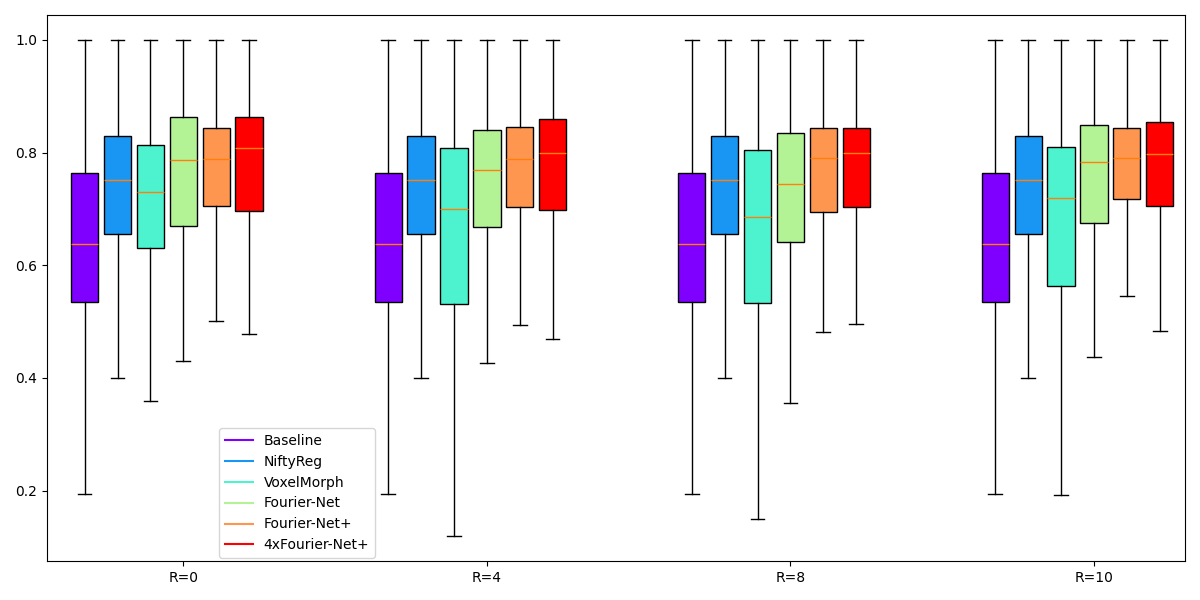
\includegraphics[width=\textwidth]{Boxplot_DiceScores_LV-Cavity.png}
    		\caption{Boxplot of the Dice scores for the left ventricle cavity.} %on the fully sampled \emph{ACDC} test data
    		\label{fig:Boxplot_DiceScores_LV-Cavity}
	\end{subfigure}
	\\
	\begin{subfigure}{0.8\textwidth}
    		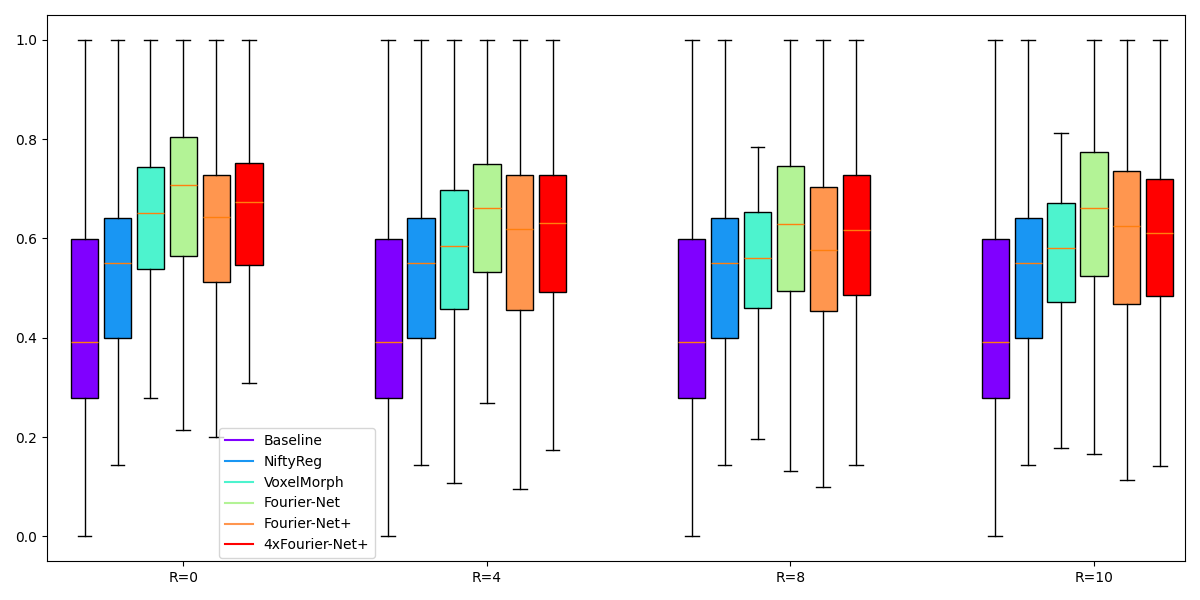
\includegraphics[width=\textwidth]{Boxplot_DiceScores_Myocardium.png}
    		\caption{Boxplot of the Dice scores for the myocardium.} %on the Acc4 \emph{ACDC} test data
    		\label{fig:Boxplot_DiceScores_Myocardium}
	\end{subfigure}
	\\
	\begin{subfigure}{0.8\textwidth}
    		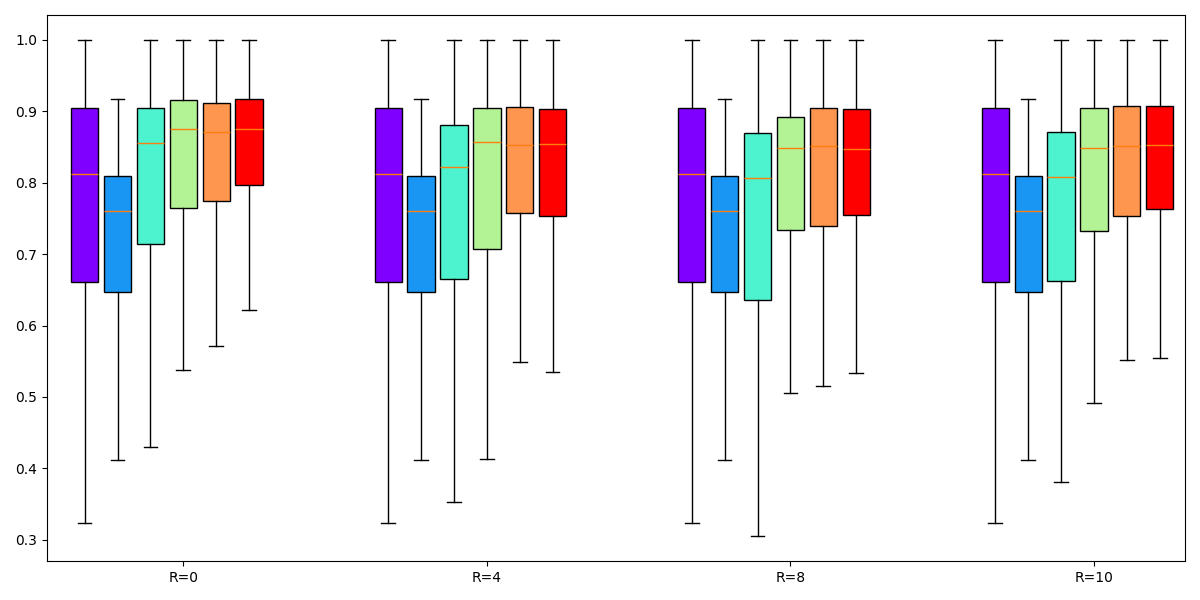
\includegraphics[width=\textwidth]{Boxplot_DiceScores_RV-Cavity.png}
    		\caption{Boxplot of the Dice scores for right ventricle cavity.} %on the Acc8 \emph{ACDC} test data
    		\label{fig:Boxplot_DiceScores_RV-Cavity}
	\end{subfigure}
	\caption{Boxplots of Dice scores (split by label excluding the background) for all models on fully sampled ($R=0$) and subsampled ($R=4$, $R=8$, $R=10$) \emph{ACDC} test data.}
	\label{fig:Boxplots_DiceScores}
\end{figure}

%\begin{figure}[h] %tpb
%	\centering
%	\graphicspath{{images/}{\main/images/}}
%	\begin{subfigure}{\textwidth}
%    		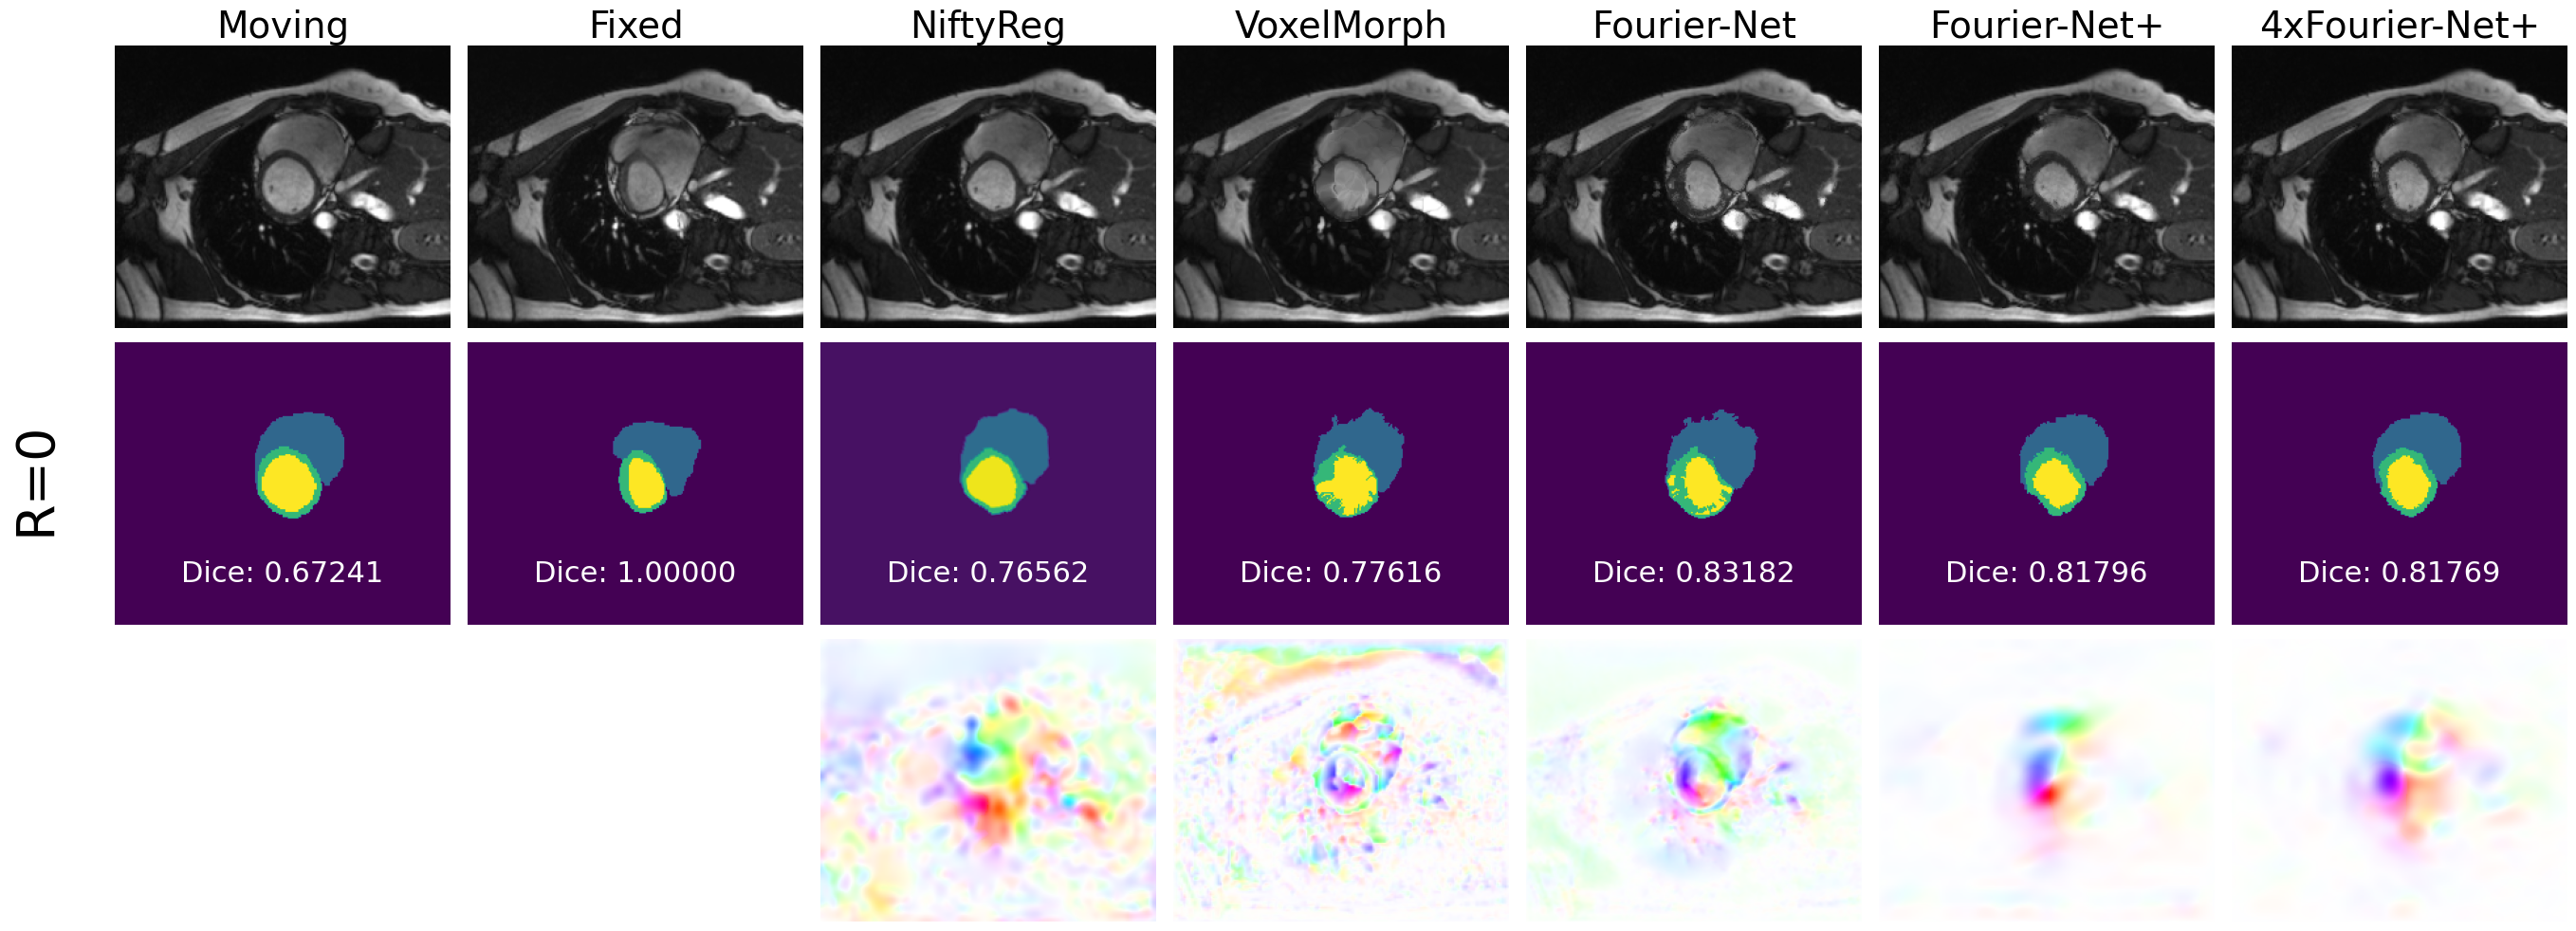
\includegraphics[width=\textwidth]{TestExamples_Mode0.png}
%    		\caption{Example images and segmentations for fully sampled ($R=0$) data.}
%    		\label{fig:TestExamples_Mode0}
%	\end{subfigure}
%	\\
%	\begin{subfigure}{\textwidth}
%    		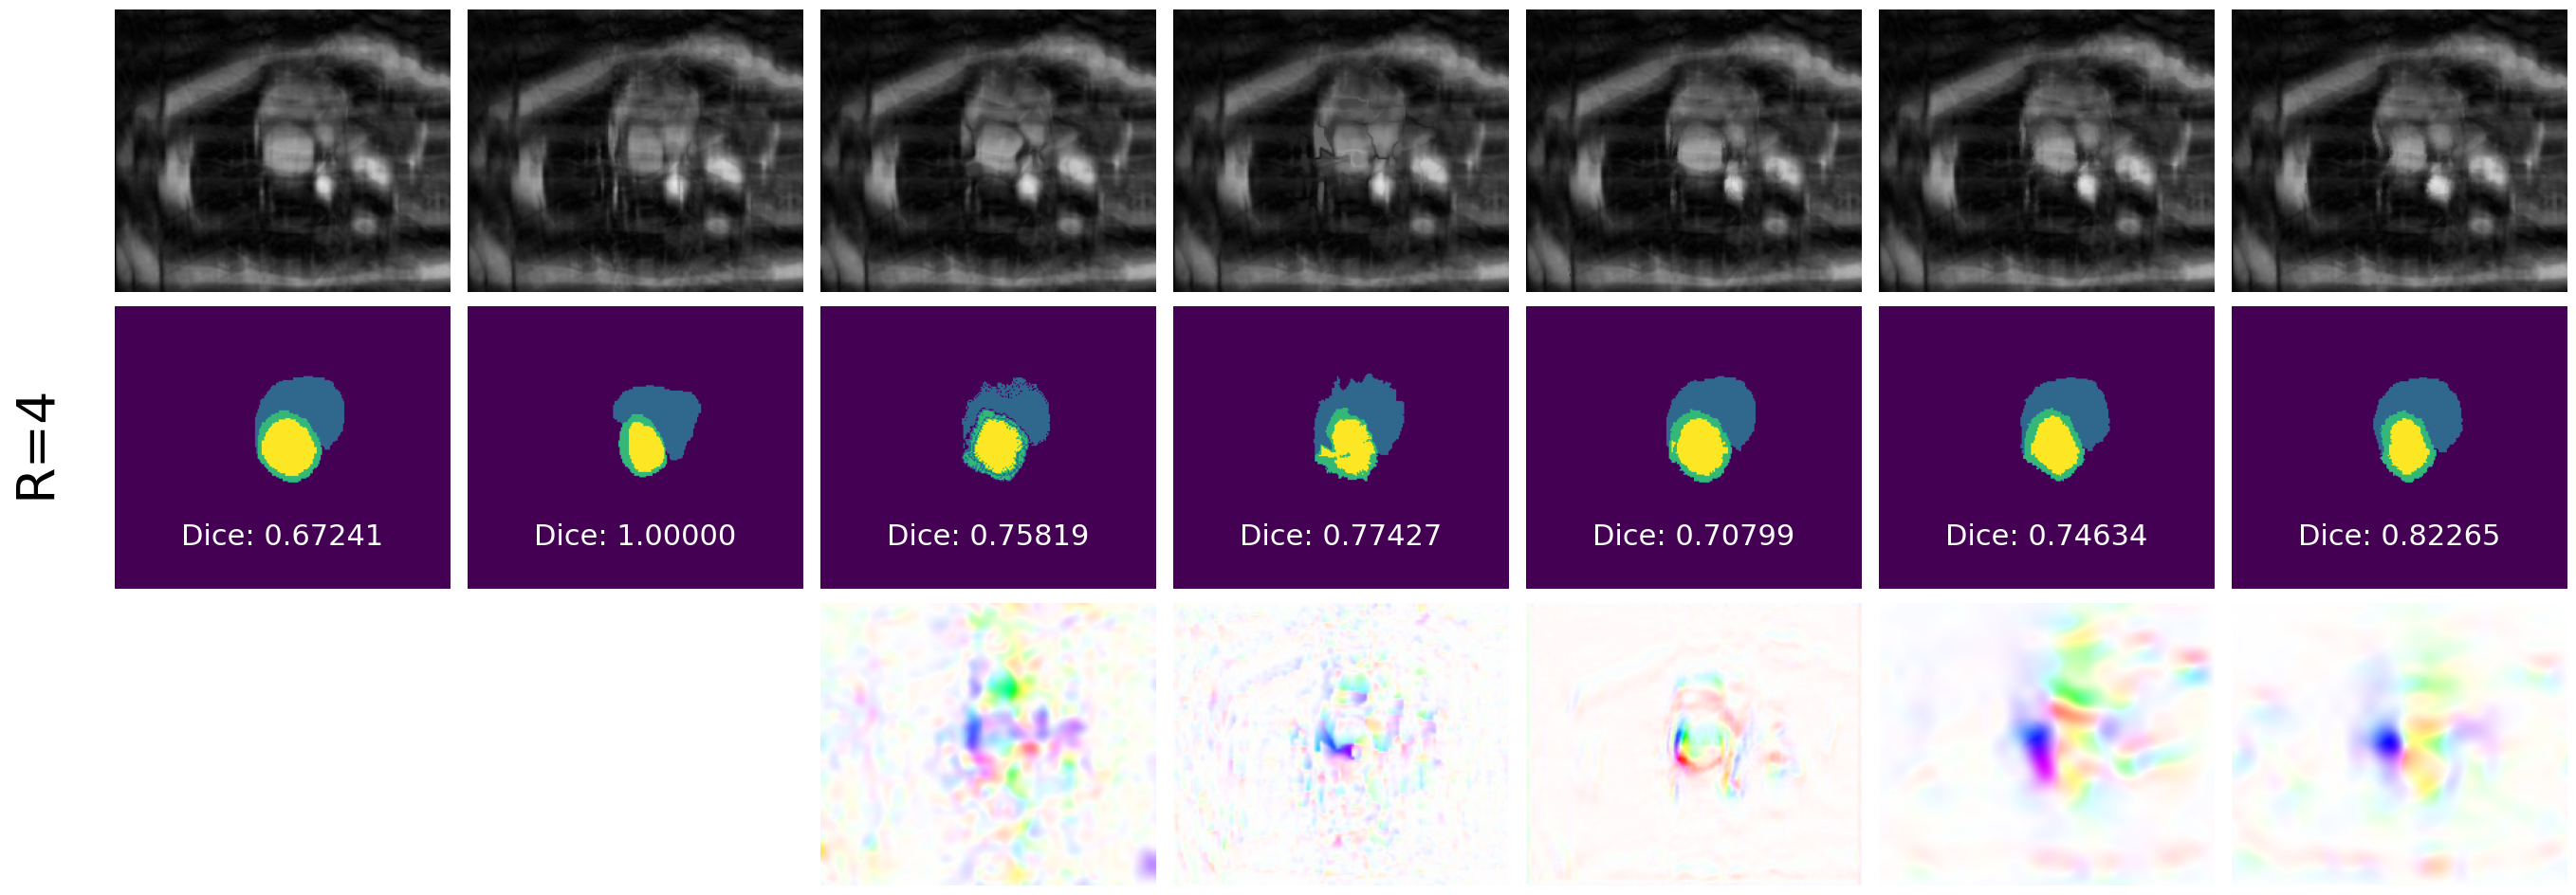
\includegraphics[width=\textwidth]{TestExamples_Mode1.png}
%    		\caption{Example images and segmentations for Acc4 ($R=4$) data.}
%    		\label{fig:TestExamples_Mode1}
%	\end{subfigure}
%	\\
%	\begin{subfigure}{\textwidth}
%    		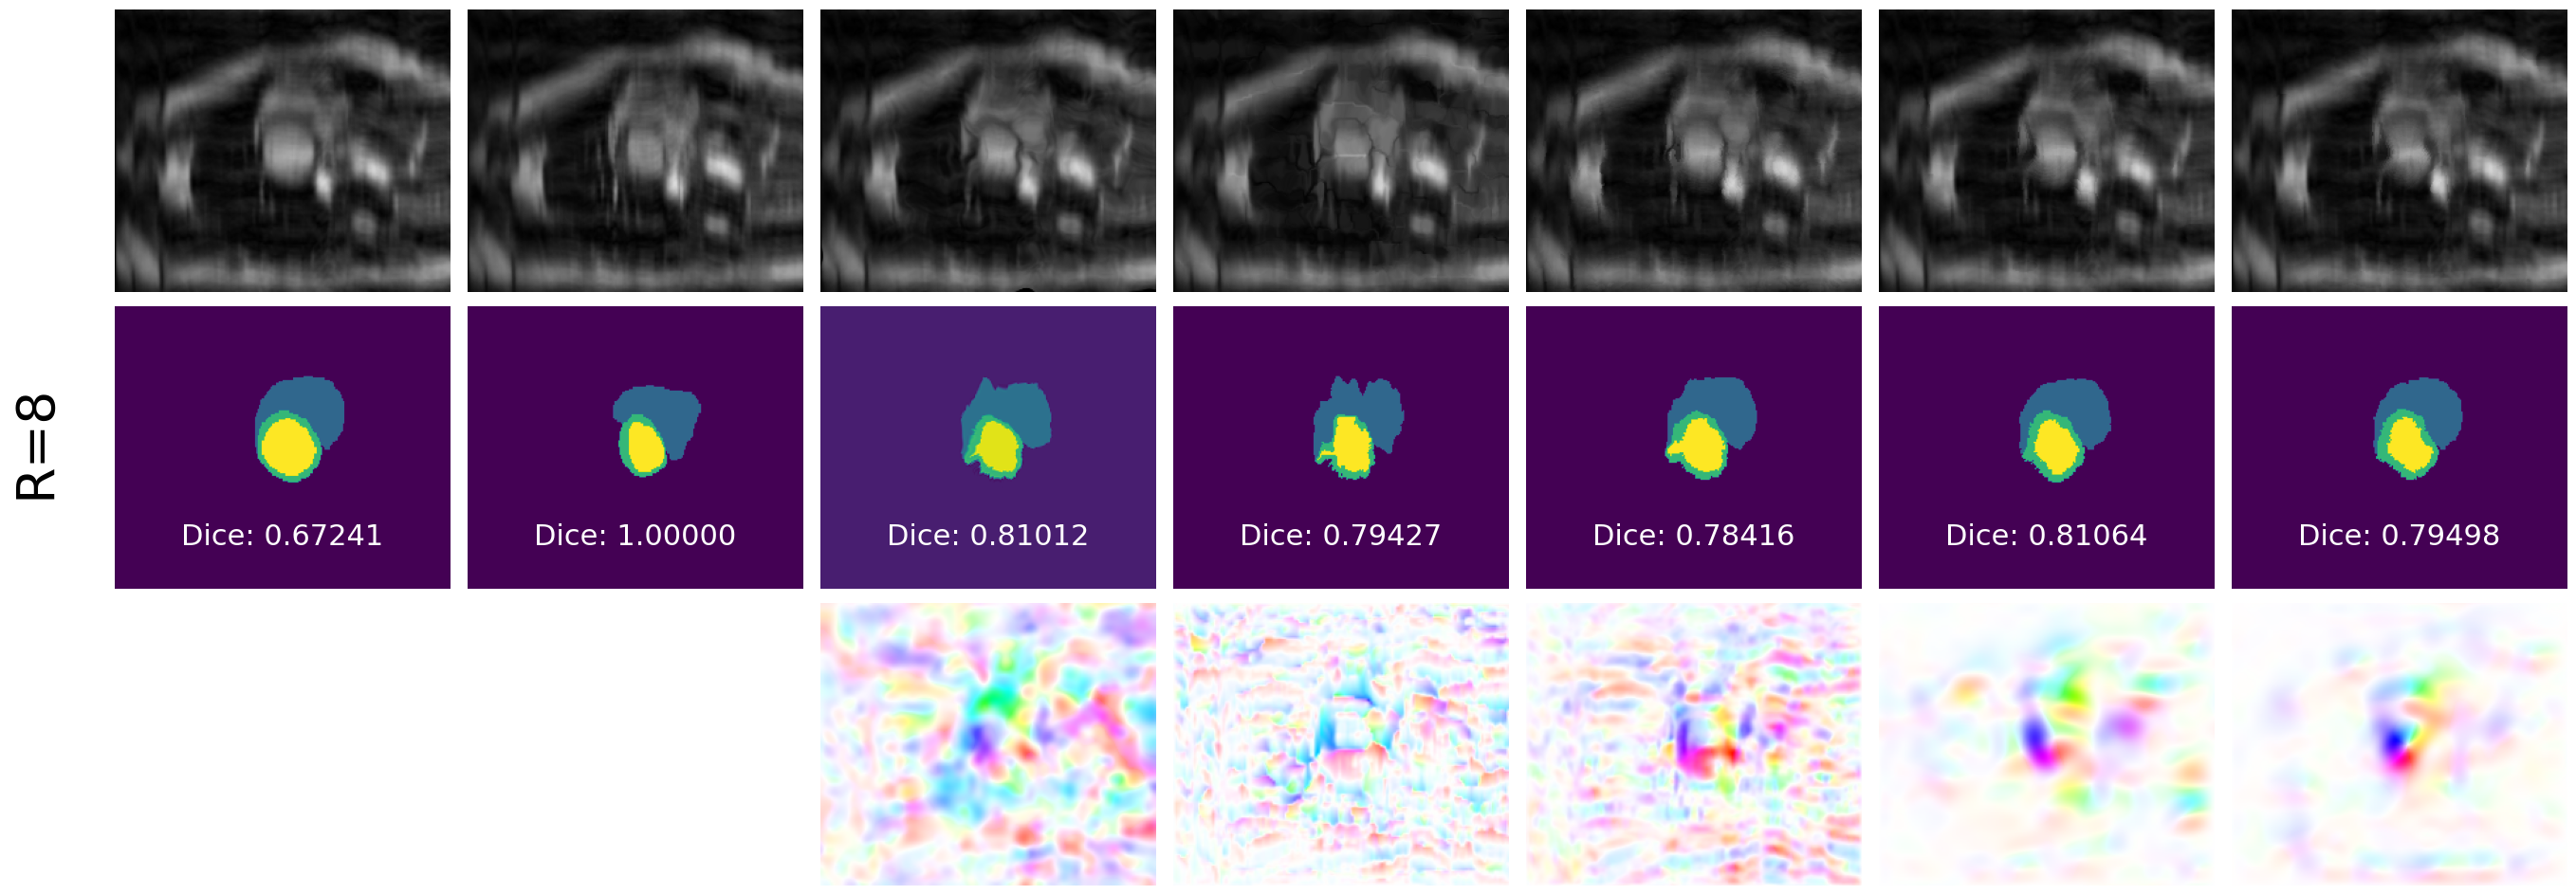
\includegraphics[width=\textwidth]{TestExamples_Mode2.png}
%    		\caption{Example images and segmentations for Acc8 ($R=8$) data.}
%    		\label{fig:TestExamples_Mode2}
%	\end{subfigure}
%	\\
%	\begin{subfigure}{\textwidth}
%    		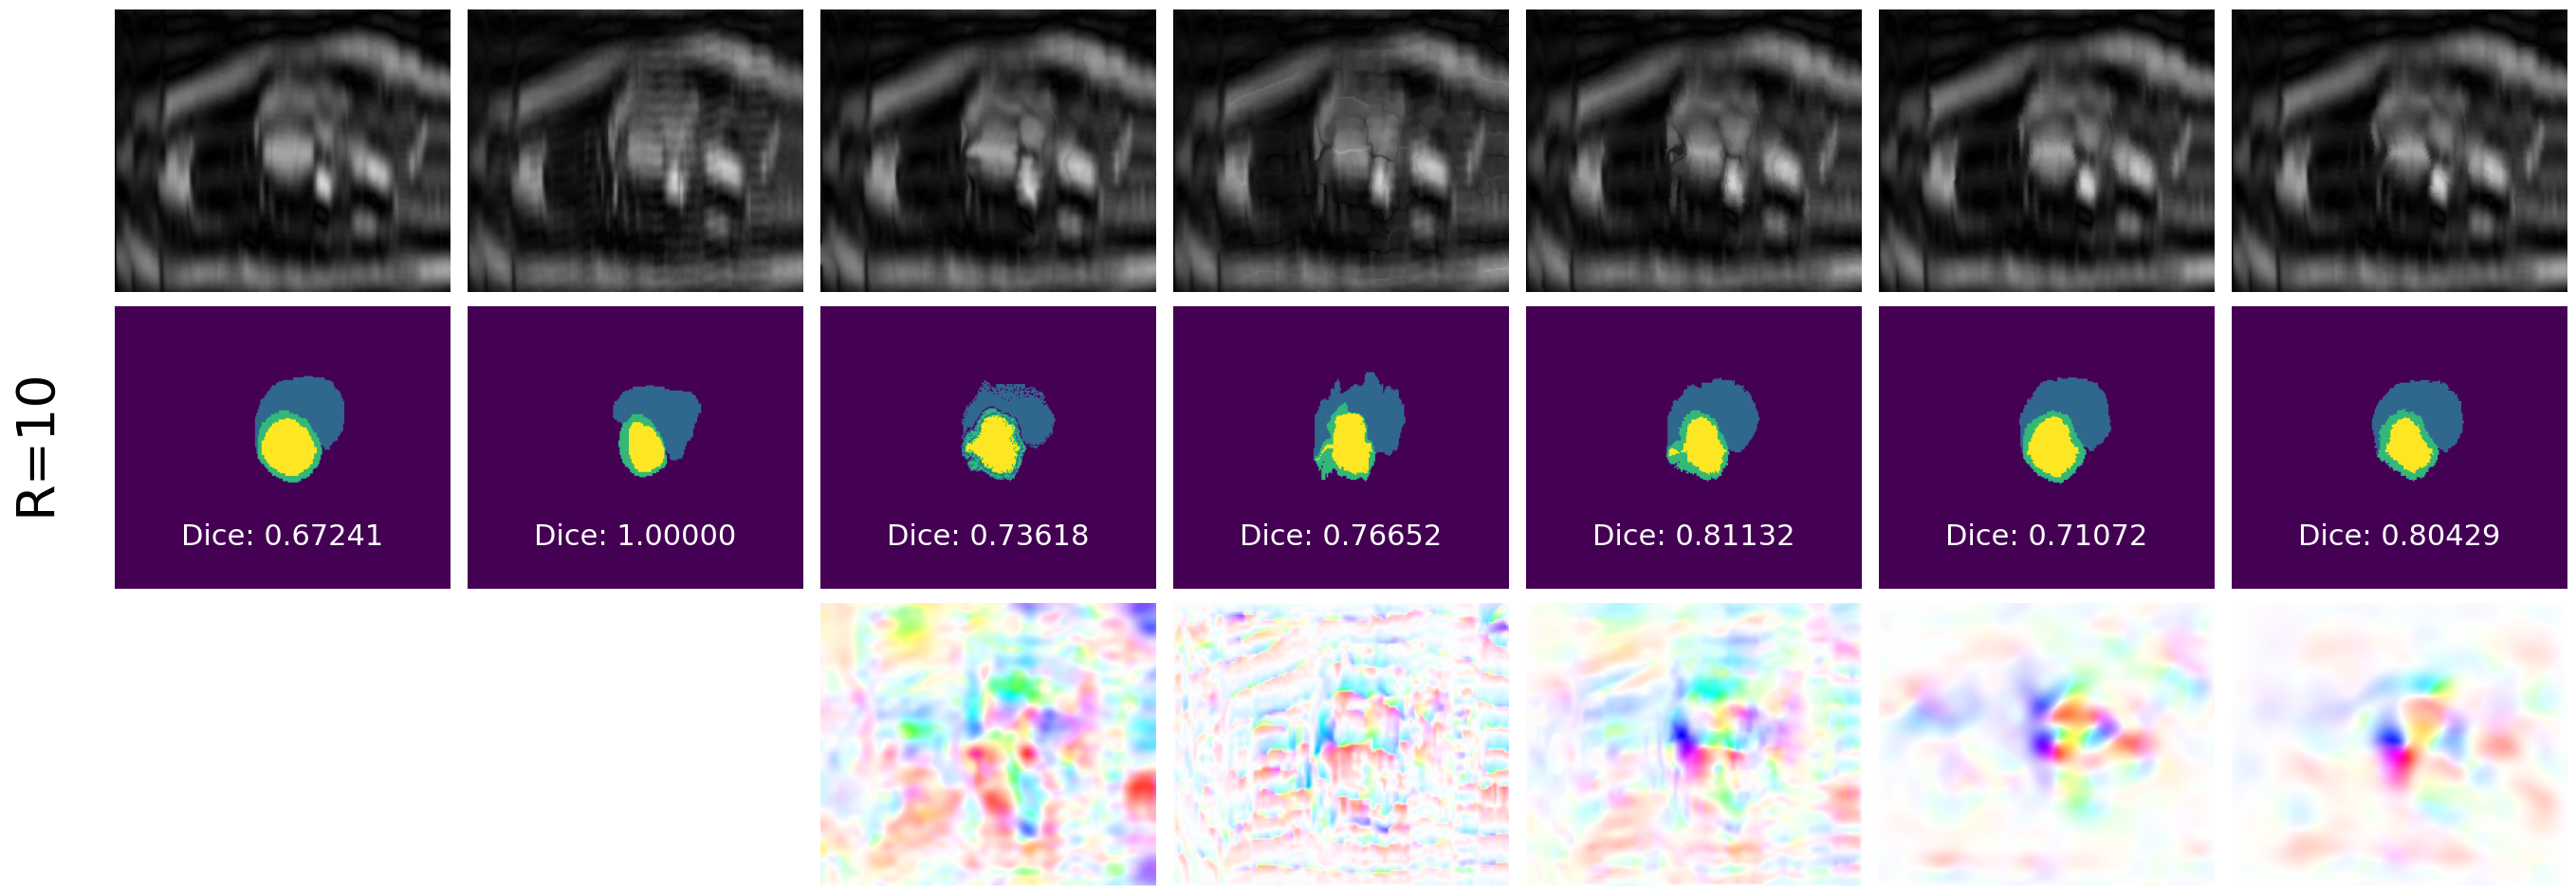
\includegraphics[width=\textwidth]{TestExamples_Mode3.png}
%    		\caption{Example images and segmentations for Acc10 ($R=10$) data.}
%    		\label{fig:TestExamples_Mode3}
%	\end{subfigure}
%	\caption{Examples of warped images and segmentations for \emph{NiftiReg}, \emph{VoxelMorph}, \emph{Fourier-Net}, \emph{Fourier-Net+} and \emph{4xFourier-Net+} together with the original image pair from the \emph{ACDC} test data.}
%	\label{fig:TestExamples}
%\end{figure}


\subsubsection{Visual Examination}
In order to explain the differences observed previously a visual examination can be useful. There one can look at the warped images and segmentations as well as the generated displacement fields visualized in Figure~\ref{fig:TestExamples}. For all acceleration factors, an example moving and fixed image can be compared to the warped images by the different methods. For further analysis, the corresponding segmentations (with Dice scores) and displacement fields for the methods are given.\\
For $R=0$, it is apparent that \emph{Fourier-Net+} and \emph{4xFourier-Net+} have very localized displacements centered on the cardiac region leading to a very smooth warped segmentation compared to \emph{Fourier-Net} and \emph{VoxelMorph} were the cardiac labels mix in some regions. Thus those networks have learned a less localized transformation, which can also be seen in the displacements. However, despite this \emph{Fourier-Net} still achieves the best Dice score with about $16\%$ increase compared to the baseline. While \emph{NiftyReg} does produce a very smooth warped segmentation the actual displacement is very small and not localized on the cardiac region leading to the worst Dice score of all methods.\\
For $R=4$, the image artifacts due to the subsampling are very apparent. The segmentations for the moving and fixed image obviously remain the same.
% despite the subsampling.
\emph{Fourier-Net+} and \emph{4xFourier-Net+} again have very smooth segmentations, however the displacements reflect the difficulties of adapting to subsampled data in becoming slightly less local. Surprisingly, \emph{NiftyReg} actually has a more localized displacement compared to the fully sampled data, however the segmentation looks less smooth and the Dice score is slightly lower. Somewhat similar, \emph{VoxelMorph} also has a more localized displacement leading to a smoother segmentation and a higher Dice score. The results of \emph{Fourier-Net} look overall very similar to the fully sampled case, perhaps with a bit more localized displacement leading to a smoother segmentation, although this does not lead to a better Dice Score.\\
For $R=8$, the displacements for all methods become more global due to the strong presence of image artifacts, however the Dice scores are better than before for all methods. \emph{NiftyReg} even outperforms \emph{VoxelMorph} for the first time. This trend does not continue for $R=10$, were \emph{NiftyReg} is again far behind all other methods in terms of Dice with a very much global displacement. \emph{VoxelMorph} seems to compensate more for the rippling artifacts present in the fixed image than for the change in the cardiac region as seen in the displacement. \emph{Fourier-Net}, \emph{Fourier-Net+} and \emph{4xFourier-Net+} do not share this behavior although their displacements also become more global and less focused on the cardiac region. The latter network performs best for the first time managing an increase in Dice of about $16\%$ compared to the baseline for this specific case despite the heavy subsampling showing the robustness of the network.

\begin{figure}[H]
	\centering
	\graphicspath{{images/}{\main/images/}}
	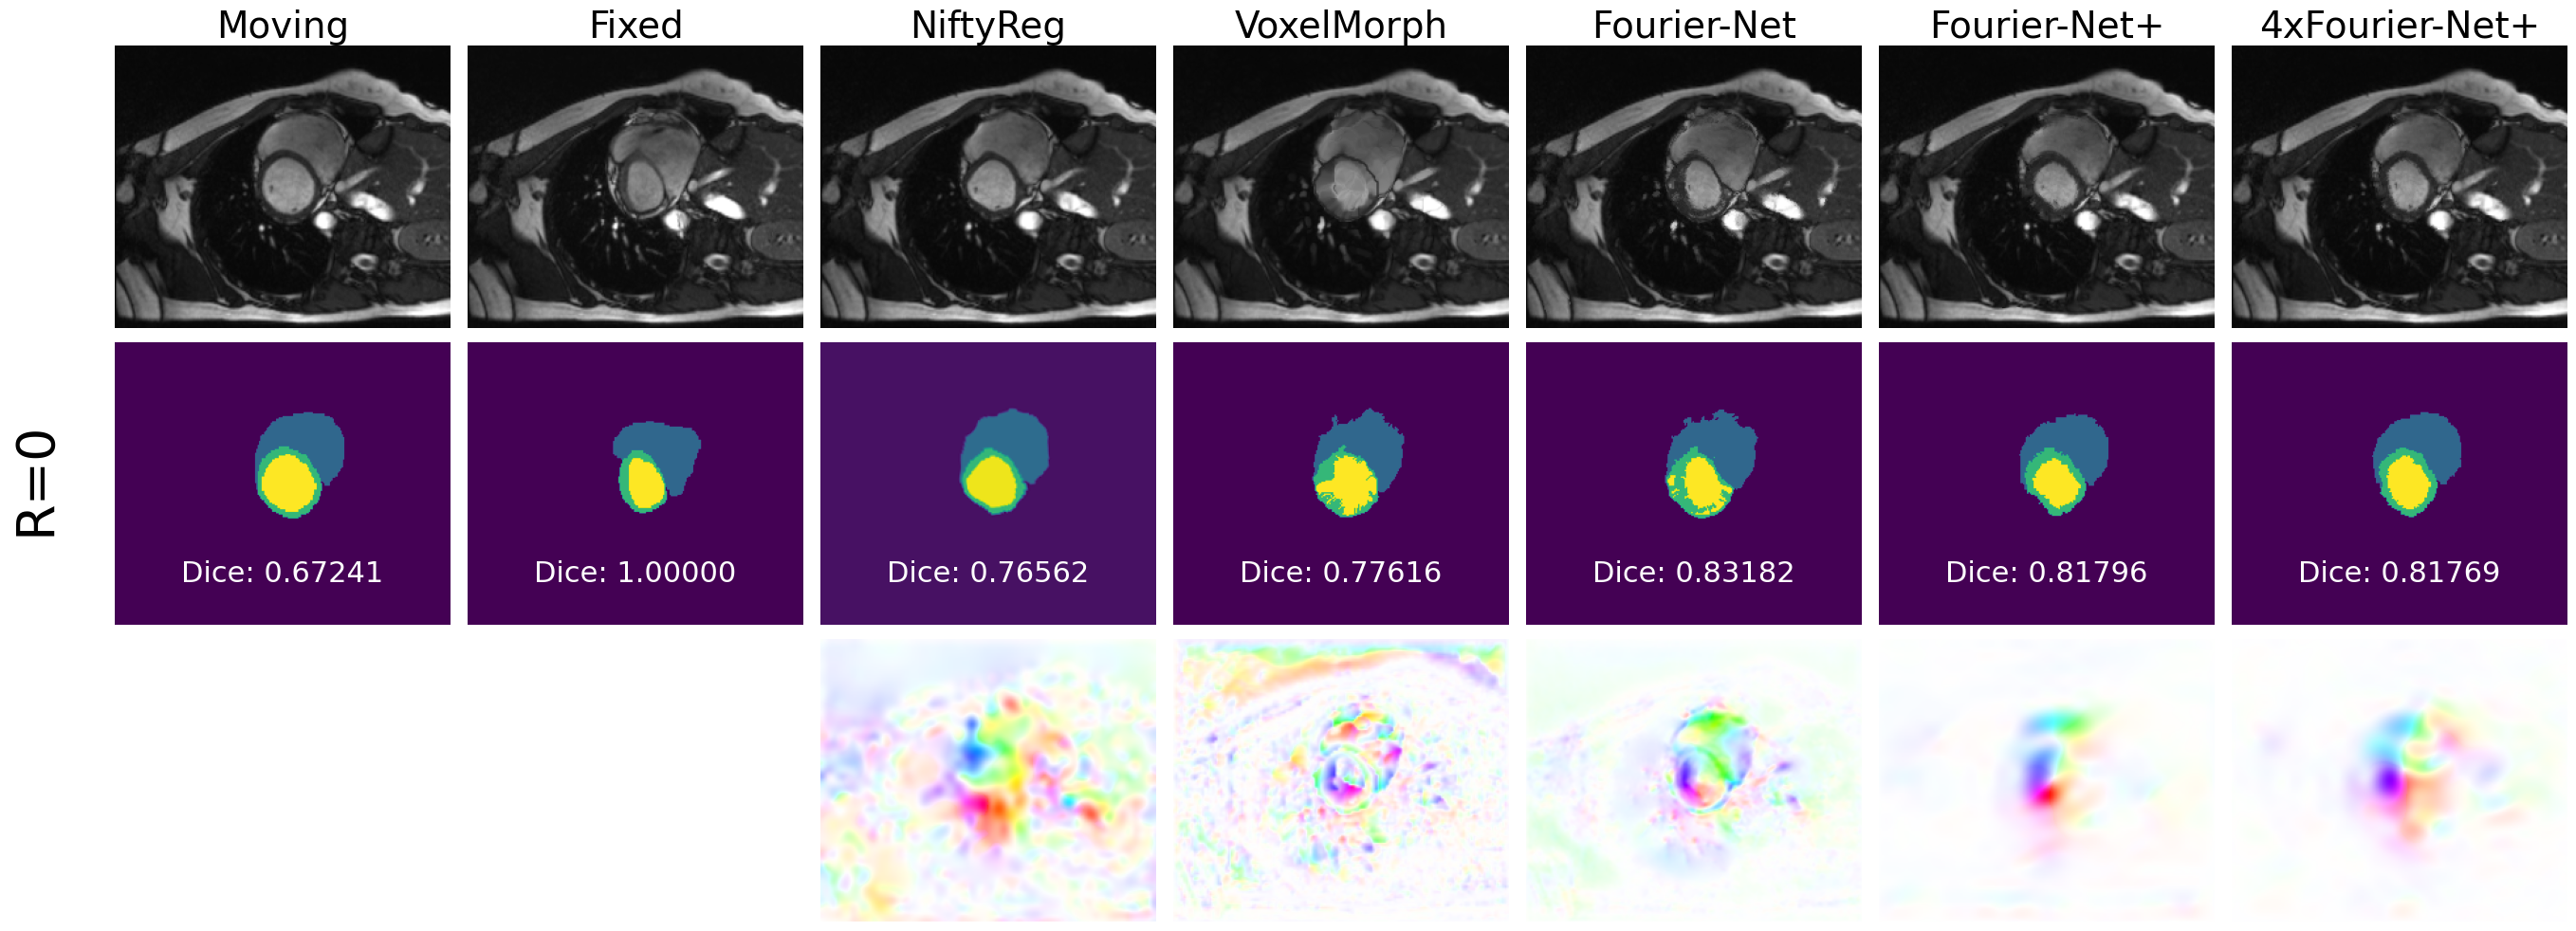
\includegraphics[width=\textwidth]{TestExamples_Mode0.png}
    	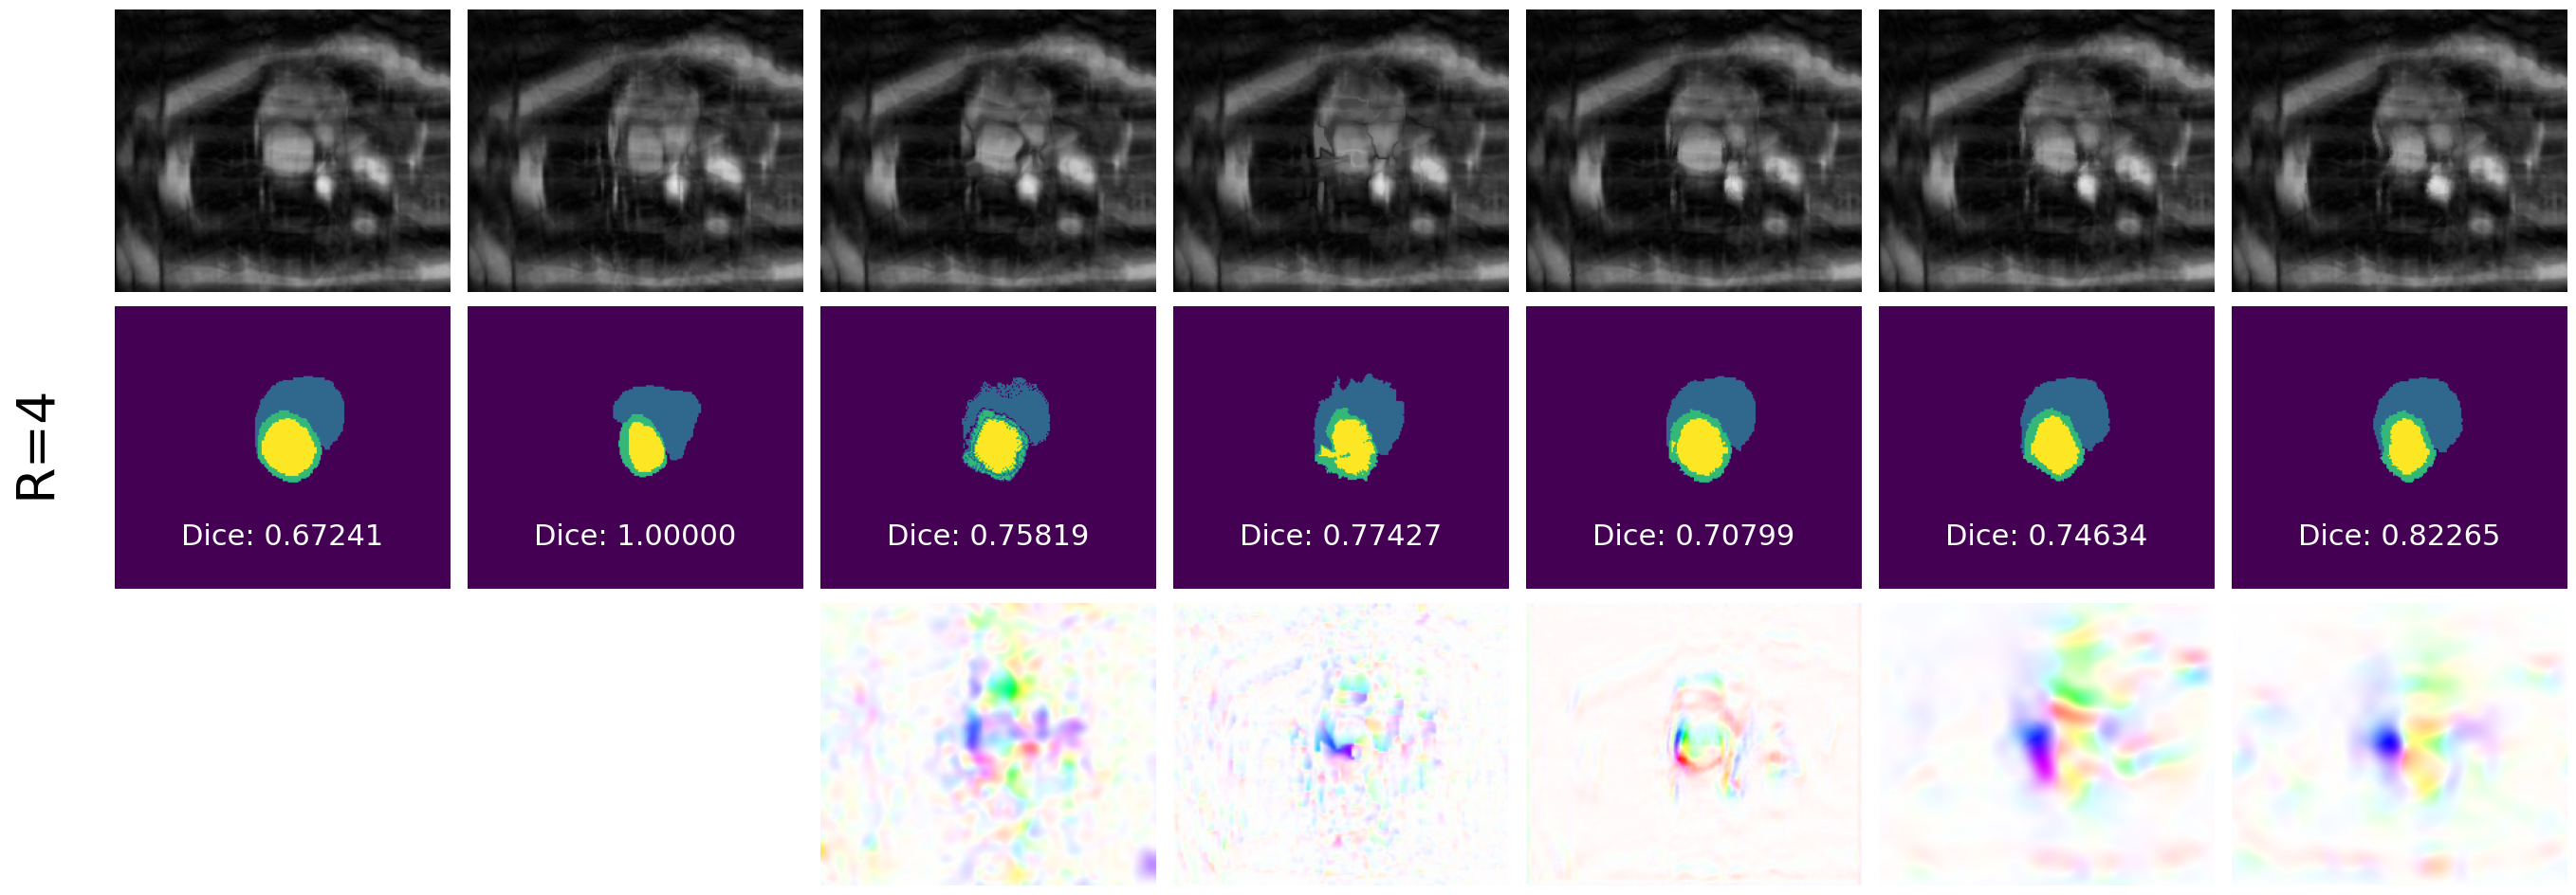
\includegraphics[width=\textwidth]{TestExamples_Mode1.png}
    	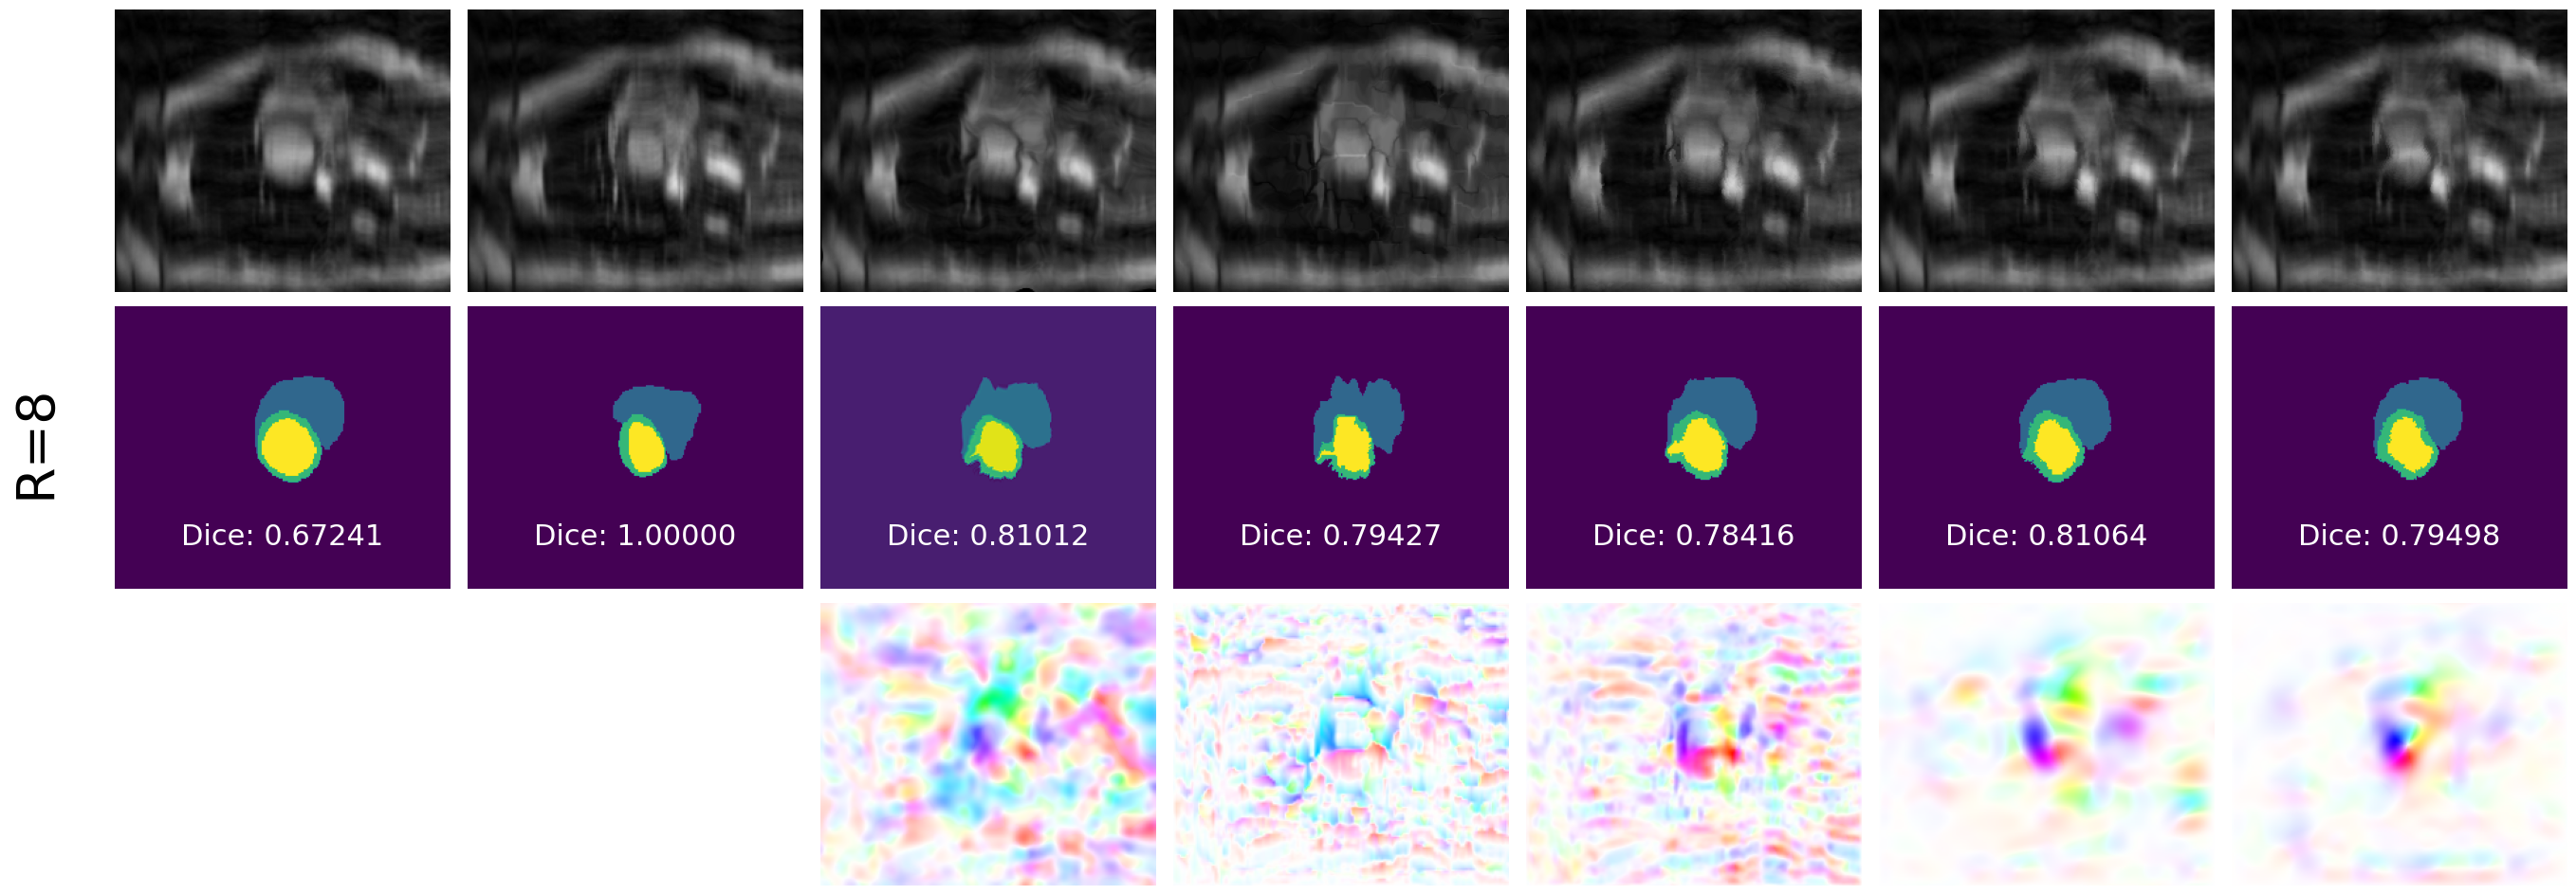
\includegraphics[width=\textwidth]{TestExamples_Mode2.png}
    	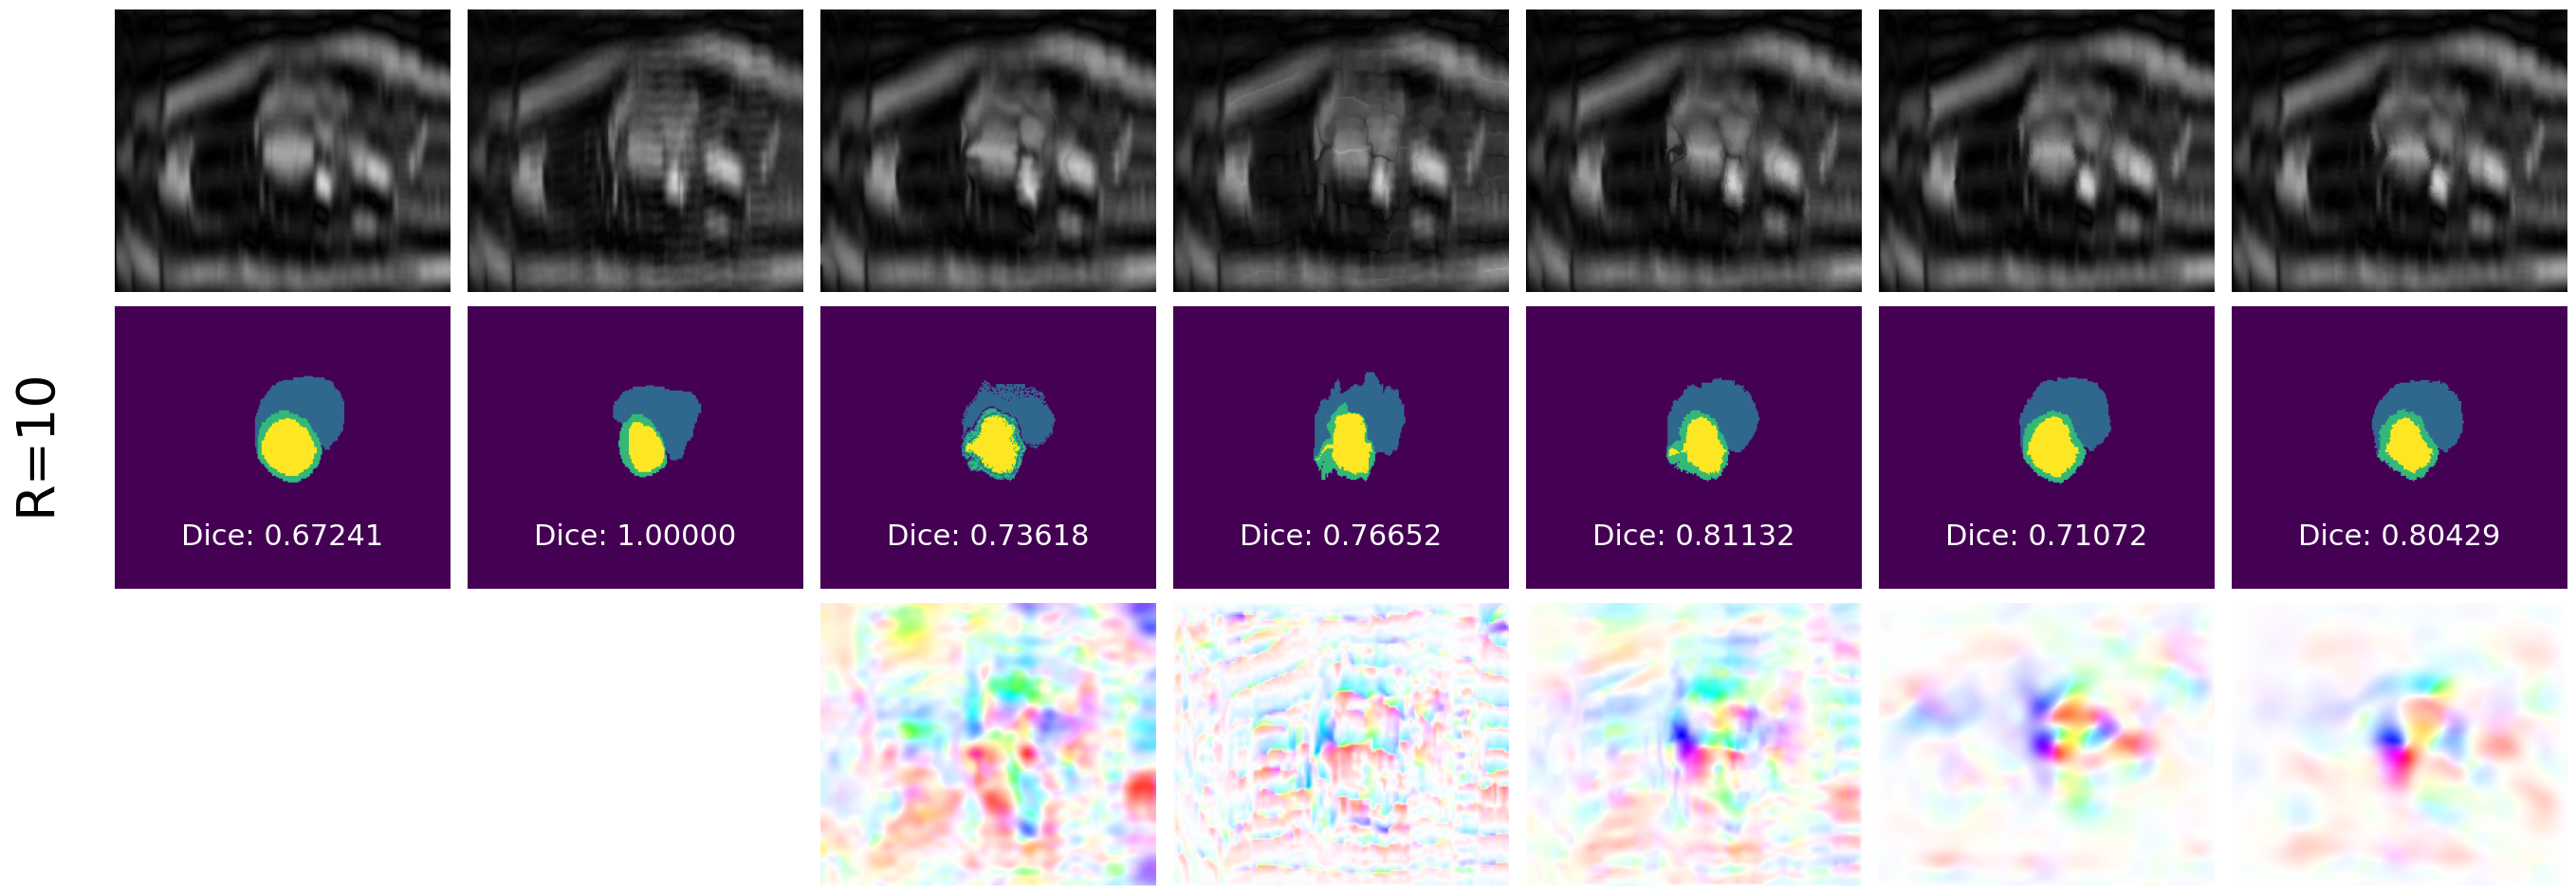
\includegraphics[width=\textwidth]{TestExamples_Mode3.png}	
	\caption{Examples of warped images, segmentations and flow fields for \emph{NiftiReg}, \emph{VoxelMorph}, \emph{Fourier-Net}, \emph{Fourier-Net+} and \emph{4xFourier-Net+} together with the original image pair from the fully sampled ($R=0$) and subsampled ($R=4$, $R=8$, $R=10$) \emph{ACDC} test data.}
	\label{fig:TestExamples}
\end{figure}


\section{Integration into a Motion-Compensated Reconstruction Pipeline} \label{Sec:ResultsIntegrationMotion-CompensatedReconstructionPipeline}
After assessing the registration performance of \emph{Fourier-Net}, \emph{Fourier-Net+} and \emph{4xFourier-Net+}, a final down-stream task to gauge the applicability of these networks was conducted in the form of an motion-compensated reconstruction pipeline where the networks are used to correct the moment between frames.

\subsection{Domain Translation} \label{SubSec:ResultsDomainTranslation}
First, the domain gap between the \emph{ACDC} and \emph{CMRxRecon} dataset was of interest. To estimate the generalizability of our previous results on the new cardiac dataset 
\emph{Fourier-Net}, \emph{Fourier-Net+} and \emph{4xFourier-Net+} were trained again on the accelerated \emph{CMRxRecon} data. They were then compared to the \emph{Fourier-Net}, \emph{Fourier-Net+} and \emph{4xFourier-Net+} version which were previously trained for 6 epochs on \emph{ACDC}. All other network parameters were held constant for comparability. The results can be seen in Table~\ref{tab:DomainTranslation_ACDC_CMRxRecon}.\\
For ...

\begin{table}[H] %tpb
	%\scriptsize
	\centering
	\caption{Results for \emph{Fourier-Net}, \emph{Fourier-Net+} and \emph{4xFourier-Net+} trained on the $R=4$ \emph{ACDC} and \emph{CMRxRecon} data and tested on the $R=4$ \emph{CMRxRecon} test data.}
	\label{tab:DomainTranslation_ACDC_CMRxRecon}
	\begin{tabular}{c c c c} %
		\toprule
		\multirow{2}{*}{Metrics} & \multicolumn{3}{c}{Trained on \emph{ACDC}} \\
		\cmidrule(lr){2-4} 
		 & Fourier-Net & Fourier-Net+ & 4xFourier-Net+\\	
		\midrule
		$\%$ SSIM & $98.21 \pm 1.07$ & $97.88 \pm 1.04$ & $97.88 \pm 1.04$\\
		MSE (m) & $0.01 \pm 0.01$ & $0.01 \pm 0.01$ & $0.01 \pm 0.01$ \\
		$\% \, |J_{\phi}|\leq0$ & $0.03 \pm 0.09$ & $0.00 \pm 0.00$ & $0.00 \pm 0.00$ \\
		Time [s] 	  & 0.0038 & 0.0037 & 0.0185  \\
		\midrule
		\multirow{2}{*}{Metrics} & \multicolumn{3}{c}{Trained on \emph{CMRxRecon}} \\
		\cmidrule(lr){2-4} 
		 & Fourier-Net & Fourier-Net+ & 4xFourier-Net+\\		
		\midrule
		$\%$ SSIM & $97.99 \pm 1.04$ & $97.88 \pm 1.06$ & $97.88 \pm 1.07$\\
		MSE (m) & $0.01 \pm 0.01$ & $0.01 \pm 0.01$ & $0.01 \pm 0.01$ \\
		$\% \, |J_{\phi}|\leq0$ & $0.00 \pm 0.01$ & $0.00 \pm 0.00$ & $0.00 \pm 0.00$ \\
		Time [s] 	  & 0.0029 & 0.0043 & 0.0120  \\
		\bottomrule
	\end{tabular}	
\end{table}

\subsection{Reconstruction Pipeline} \label{SubSec:ResultsReconstructionPipeline}
After ensuring that the previous results were translatable to the new data, the reconstruction pipeline had to be evaluated. As the \emph{CMRxRecon} dataset does not include segmentations for Dice calculation, image similarity metrics need to be utilized. For this, SSIM and MSE were used again, however, the PSNR (see section~\ref{SubSubSec:TestingEvalutionMetrics}) and HaarPSI~\cite{HaarPSI} were also added. 

\subsubsection{K-Space Line Swapping}
After ensuring that the reconstruction pipeline worked, the input images were further corrupted as the cardiac motion present was not deemed severe enough. To simulate motion or mis-triggering a similar strategy to~\cite{Oksuz2020} was used, swapping $z=\{16,32\}$ k-space lines between the frames. Results for the motion-compensated reconstruction using \emph{VoxelMorph}, \emph{Fourier-Net}, \emph{Fourier-Net+} and \emph{4xFourier-Net+} is shown in Table~\ref{tab:ComparisonReconstructionCMRxRecon} with blue marking the best results per metric (not present if all methods have the same performance) and red marking worse results than the baseline.\\
For $z=16$, performance decreases with higher acceleration. For $R=4$, \emph{Fourier-Net} has the highest HaarPSI and SSIM values, while \emph{VoxelMorph} has the highest PSNR. \emph{Fourier-Net+} on the other hand, has the lowest values for these metrics. All methods as well as the baseline have the same mean MSE value. Only for the third decimal point in the standard deviation a small difference between the different methods is visible (note that the MSE values are already multiplied by a factor of 100).%\\
For $R=8$, \emph{Fourier-Net} again has the highest value for the HaarPSI, followed by \emph{Fourier-Net+}, as well as the highest SSIM value, followed by \emph{4xFourier-Net+} which also has the highest PSNR. While the MSE values are again very close, \emph{4xFourier-Net+} has a slightly lower mean value than the other methods.%\\
For $R=10$, \emph{4xFourier-Net+} performs best for all metrics with \emph{Fourier-Net+} having the same mean MSE value. \emph{VoxelMorph} and \emph{Fourier-Net} perform worse than baseline for the HaarPSI with the latter also having lower PSNR and SSIM values than the baseline.\\
For $z=32$ and $R=4$, \emph{Fourier-Net} performs best for all metrics, while \emph{4xFourier-Net+} performs worse than baseline for PSNR, SSIM and MSE. For $R=8$, \emph{Fourier-Net+} has the highest HaarPSI, PSNR and SSIM values followed by \emph{Fourier-Net}. The mean MSE value is again the same for all methods and slightly lower than the baseline. For $R=10$, \emph{Fourier-Net+} again performs best for all metrics. Only \emph{Fourier-Net} has a lower SSIM than the baseline.

\begin{table}[h] %tpb
	\footnotesize
	\centering
	\caption{Reconstruction results \emph{VoxelMorph}, \emph{Fourier-Net}, \emph{Fourier-Net+} and \emph{4xFourier-Net+} on the \emph{CMRxRecon} test data for $R=4$, $R=8$ and $R=10$ as well as an baseline without motino-correction. The best results for each metric and subsampling are highlighted in blue, while values worse than the unaligned baseline are marked with red.}
	\label{tab:ComparisonReconstructionCMRxRecon}
	\begin{tabular}{c c c c c c} 
		\toprule
		 & \multirow{2}{*}{Methods} & \multicolumn{4}{c}{Motion-correction for $z=16$ swapped k-space lines} \\
		\cmidrule(lr){3-6} 
		 & & $\%$ HaarPSI & PSNR [dB] & $\%$ SSIM & MSE (m)\\
		
		% 4x Accelerated (R=4) 				 		
		\midrule
		\multirow{5}{*}{\rotatebox{90}{$R=4$}} & Baseline & $56.884 \pm 8.129$ & $28.703 \pm 2.388$ & $78.079 \pm 5.887$ & $0.160 \pm 0.125$ \\  
		 & VoxelMorph & $56.909 \pm 8.118$ & \textcolor{blue}{$28.709 \pm 2.404$} & $78.090 \pm 5.903$ & $0.160 \pm 0.126$ \\  
		 & Fourier-Net & \textcolor{blue}{$56.918 \pm 8.160$} & $28.706 \pm 2.401$ & \textcolor{blue}{$78.123 \pm 5.893$} & $0.160 \pm 0.126$ \\  
		 & Fourier-Net+ & \textcolor{red}{$56.854 \pm 8.158$} & \textcolor{red}{$28.699 \pm 2.399$} & \textcolor{red}{$78.071 \pm 5.951$} & $0.160 \pm 0.126$ \\   
		 & 4xFourier-Net+ & $56.903 \pm 8.109$ & $28.702 \pm 2.380$ & $78.085 \pm 5.877$ & $0.160 \pm 0.125$ \\  
		
		% 8x Accelerated (R=8) 
		\midrule
		\multirow{5}{*}{\rotatebox{90}{$R=8$}} & Baseline & $53.318 \pm 7.641$ & $28.104 \pm 2.383$ & $77.311 \pm 5.934$ & $0.183 \pm 0.139$ \\  
		 & VoxelMorph & $53.342 \pm 7.687$ & $28.110 \pm 2.405$ & $77.341 \pm 5.900$ & $0.183 \pm 0.139$ \\  
		 & Fourier-Net & \textcolor{blue}{$53.394 \pm 7.681$} & $28.128 \pm 2.398$ & \textcolor{blue}{$77.416 \pm 5.927$} & $0.183 \pm 0.138$ \\  
		 & Fourier-Net+ & $53.388 \pm 7.664$ & $28.118 \pm 2.404$ & $77.398 \pm 5.906$ & $0.183 \pm 0.138$ \\   
		 & 4xFourier-Net+ & $53.376 \pm 7.688$ & \textcolor{blue}{$28.133 \pm 2.398$} & $77.402 \pm 5.936$ & \textcolor{blue}{$0.182 \pm 0.138$} \\ 
		 	 
		% 10x Accelerated (R=10) 		 		
		\midrule		
		\multirow{5}{*}{\rotatebox{90}{$R=10$}} & Baseline & $52.212 \pm 7.388$ & $27.906 \pm 2.364$ & $77.175 \pm 5.886$ & $0.191 \pm 0.141$ \\  
		 & VoxelMorph & \textcolor{red}{$52.211 \pm 7.393$} & $27.907 \pm 2.368$ & $77.194 \pm 5.863$ & $0.191 \pm 0.140$ \\  
		 & Fourier-Net & \textcolor{red}{$52.192 \pm 7.361$} & \textcolor{red}{$27.895 \pm 2.362$} & \textcolor{red}{$77.160 \pm 5.815$} & $0.191 \pm 0.139$ \\  
		 & Fourier-Net+ & $52.240 \pm 7.379$ & $27.924 \pm 2.357$ & $77.244 \pm 5.866$ & \textcolor{blue}{$0.189 \pm 0.139$} \\   
		 & 4xFourier-Net+ & \textcolor{blue}{$52.272 \pm 7.330$} & \textcolor{blue}{$27.931 \pm 2.349$} & \textcolor{blue}{$77.262 \pm 5.816$} & \textcolor{blue}{$0.189 \pm 0.137$} \\ 
		 
		 \midrule	
		 & & \multicolumn{4}{c}{Motion-correction for $z=32$ swapped k-space lines} \\
		% 4x Accelerated (R=4) 				 		
		\midrule
		\multirow{5}{*}{\rotatebox{90}{$R=4$}} & Baseline & $52.711 \pm 7.673$ & $27.506 \pm 2.180$ & $74.379 \pm 5.869$ & $0.203 \pm 0.130$ \\  
		 & VoxelMorph & $52.747 \pm 7.658$ & $27.512 \pm 2.188$ & $74.349 \pm 5.900$ & $0.203 \pm 0.129$ \\  
		 & Fourier-Net & \textcolor{blue}{$52.802 \pm 7.708$} & \textcolor{blue}{$27.536 \pm 2.197$} & \textcolor{blue}{$74.421 \pm 5.937$} & \textcolor{blue}{$0.202 \pm 0.128$} \\  
		 & Fourier-Net+ & $52.725 \pm 7.724$ & $27.522 \pm 2.198$ & $74.366 \pm 5.892$ & $0.203 \pm 0.129$ \\   
		 & 4xFourier-Net+ & $52.711 \pm 7.718$ & \textcolor{red}{$27.500 \pm 2.205$} & \textcolor{red}{$74.353 \pm 5.986$} & \textcolor{red}{$0.204 \pm 0.132$} \\  
		
		% 8x Accelerated (R=8) 
		\midrule
		\multirow{5}{*}{\rotatebox{90}{$R=8$}} & Baseline & $50.071 \pm 7.259$ & $27.153 \pm 2.199$ & $74.033 \pm 5.844$ & $0.221 \pm 0.138$ \\  
		 & VoxelMorph & $50.091 \pm 7.301$ & $27.164 \pm 2.198$ & $74.060 \pm 5.890$ & $0.220 \pm 0.138$ \\  
		 & Fourier-Net & $50.152 \pm 7.325$ & $27.178 \pm 2.202$ & $74.094 \pm 5.826$ & $0.220 \pm 0.140$ \\  
		 & Fourier-Net+ & \textcolor{blue}{$50.159 \pm 7.362$} & \textcolor{blue}{$27.196 \pm 2.221$} & \textcolor{blue}{$74.119 \pm 5.853$} & $0.220 \pm 0.141$ \\   
		 & 4xFourier-Net+ & $50.128 \pm 7.276$ & $27.165 \pm 2.201$ & $74.054 \pm 5.842$ & $0.220 \pm 0.137$ \\ 
		 	 
		% 10x Accelerated (R=10) 		 		
		\midrule		
		\multirow{5}{*}{\rotatebox{90}{$R=10$}} & Baseline & $49.193 \pm 7.022$ & $27.013 \pm 2.170$ & $73.971 \pm 5.788$ & $0.227 \pm 0.143$ \\  
		 & VoxelMorph & $49.241 \pm 7.047$ & $27.026 \pm 2.179$ & $73.976 \pm 5.795$ & $0.227 \pm 0.142$ \\  
		 & Fourier-Net & $49.255 \pm 7.011$ & $27.024 \pm 2.168$ & \textcolor{red}{$73.952 \pm 5.793$} & $0.227 \pm 0.141$ \\  
		 & Fourier-Net+ & \textcolor{blue}{$49.296 \pm 7.001$} & \textcolor{blue}{$27.045 \pm 2.172$} & \textcolor{blue}{$74.028 \pm 5.784$} & \textcolor{blue}{$0.226 \pm 0.140$} \\   
		 & 4xFourier-Net+ & $49.287 \pm 7.066$ & $27.032 \pm 2.176$ & $74.022 \pm 5.820$ & $0.227 \pm 0.143$ \\ 
		 \bottomrule
	\end{tabular}
\end{table}

\subsubsection{Simulated Lung Movement}
As the results still did not look great, a second test with simulated movement was conducted. This time, multiple frames with simulated random deformations were introduced to simulate lung movement in the image, which is then to be removed with the networks.


\begin{table}[h] %tpb
	\footnotesize
	\centering
	\caption{Reconstruction results \emph{VoxelMorph}, \emph{Fourier-Net}, \emph{Fourier-Net+} and \emph{4xFourier-Net+} on the \emph{CMRxRecon} test data for $R=4$, $R=8$ and $R=10$ as well as an baseline without motino-correction. The best results for each metric and subsampling are highlighted in blue, while values worse than the unaligned baseline are marked with red.}
	\label{tab:ComparisonReconstructionCMRxRecon}
	\begin{tabular}{c c c c c c} 
		\toprule
		 & Methods & $\%$ HaarPSI & PSNR [dB] & $\%$ SSIM & MSE (m)\\
		
		% 4x Accelerated (R=4) 				 		
		\midrule
		\multirow{5}{*}{\rotatebox{90}{$R=4$}} & Baseline & $28.882 \pm 3.802$ & $23.291 \pm 1.654$ & $70.375 \pm 4.467$ & $0.504 \pm 0.197$ \\  
		 & VoxelMorph & $54.177 \pm 7.495$ & $28.347 \pm 2.369$ & $79.873 \pm 4.878$ & $0.174 \pm 0.138$ \\ 
		 & Fourier-Net & $-$ & $-$ & $-$ & $-$ \\  
		 & Fourier-Net+ & $-$ & $-$ & $-$ & $-$ \\    
		 & 4xFourier-Net+ & $-$ & $-$ & $-$ & $-$ \\ 
		
		% 8x Accelerated (R=8) 
		\midrule
		\multirow{5}{*}{\rotatebox{90}{$R=8$}} & Baseline & $28.572 \pm 3.773$ & $23.173 \pm 1.686$ & $70.603 \pm 4.533$ & $0.519 \pm 0.207$ \\  
		 & VoxelMorph & $-$ & $-$ & $-$ & $-$ \\ 
		 & Fourier-Net & $-$ & $-$ & $-$ & $-$ \\  
		 & Fourier-Net+ & $-$ & $-$ & $-$ & $-$ \\    
		 & 4xFourier-Net+ & $-$ & $-$ & $-$ & $-$ \\ 
		 	 
		% 10x Accelerated (R=10) 		 		
		\midrule		
		\multirow{5}{*}{\rotatebox{90}{$R=10$}} & Baseline & $28.486 \pm 3.766$ & $23.132 \pm 1.695$ & $70.742 \pm 4.436$ & $0.524 \pm 0.211$ \\  
		 & VoxelMorph & $-$ & $-$ & $-$ & $-$ \\ 
		 & Fourier-Net & $-$ & $-$ & $-$ & $-$ \\  
		 & Fourier-Net+ & $-$ & $-$ & $-$ & $-$ \\    
		 & 4xFourier-Net+ & $-$ & $-$ & $-$ & $-$ \\ 
		 \bottomrule
	\end{tabular}
\end{table}